% Preamble
\documentclass[12pt, twoside]{book}
\usepackage[utf8]{inputenc}
\usepackage{graphicx}
\usepackage{amsmath}
\usepackage{amsfonts}
\usepackage{nicematrix}
\usepackage{algorithm}
\usepackage{algpseudocode}
\usepackage{mathtools} % dcases

\usepackage{datetime}

\newdateformat{monthyeardate}{%
  \monthname[\THEMONTH], \THEYEAR}

\graphicspath{ {images/} }

\usepackage[a4paper,width=150mm,top=20mm,bottom=20mm,bindingoffset=6mm]{geometry}

\usepackage{fancyhdr}
\pagestyle{fancy}
\fancyhead{}
\fancyhead[RO,LE]{Towards Exascale Multiparticle Simulations}
\fancyfoot{}
\fancyfoot[LE,RO]{\thepage}
\fancyfoot[LO,CE]{Chapter \thechapter}
\fancyfoot[CO,RE]{Srinath Kailasa}

\usepackage{titlesec}

\titleformat{\chapter}[display]
  {\normalfont\bfseries}{}{0pt}{\Huge}

\usepackage[backend=bibtex]{biblatex}
\addbibresource{references.bib}


\usepackage{lipsum}
\usepackage[toc]{glossaries}

\makeglossaries
\newglossaryentry{FMM}{
    name={FMM},
    description={
    Fast Multipole Method.
    }
}

\newglossaryentry{HPC}{
    name={HPC},
    description={
        High Performance Computing.
    }
}

\newglossaryentry{flops}{
    name={flops},
    description={
        Floating Point Operations per Second.
    }
}

\newglossaryentry{API}{
    name={API},
    description={
        Application Programming Interface - the software interface to a library.
    }
}


\newglossaryentry{CPU}{
    name={CPU},
    description={
        Central Processing Unit
    }
}

% Default fixed font does not support bold face
\DeclareFixedFont{\ttb}{T1}{txtt}{bx}{n}{12} % for bold
\DeclareFixedFont{\ttm}{T1}{txtt}{m}{n}{12}  % for normal

% Custom colors
\usepackage{color}
\definecolor{deepblue}{rgb}{0,0,0.5}
\definecolor{deepred}{rgb}{0.6,0,0}
\definecolor{deepgreen}{rgb}{0,0.5,0}

\usepackage{listings}

% Python style for highlighting
\newcommand\pythonstyle{\lstset{
language=Python,
basicstyle=\ttm,
otherkeywords={self},             % Add keywords here
keywordstyle=\ttb\color{deepblue},
emph={MyClass,__init__},          % Custom highlighting
emphstyle=\ttb\color{deepred},    % Custom highlighting style
stringstyle=\color{deepgreen},
frame=tb,                         % Any extra options here
showstringspaces=false            %
}}


% Python environment
\lstnewenvironment{python}[1][]
{
\pythonstyle
\lstset{#1}
}
{}

% Python for external files
\newcommand\pythonexternal[2][]{{
\pythonstyle
\lstinputlisting[#1]{#2}}}

% Python for inline
\newcommand\pythoninline[1]{{\pythonstyle\lstinline!#1!}}

% Remove excess double page
\let\cleardoublepage\clearpage

\begin{document}


    \frontmatter

    \begin{titlepage}
    \begin{center}
        \vspace*{1cm}

        \Huge
        \textbf{Computational Topics on the Solution of Integral Equations}

        \Large
        \vspace{0.5cm}
        %Subtitle

        \vfill

        \textbf{Srinath Kailasa}

        \vspace{5cm}

        A thesis submitted in partial fulfillment of the requirements for the
        degree Doctor of Philosophy 

        \vspace{0.8cm}

        % 
\includegraphics[width=0.4\textwidth]{university.png}

        \large
        Department of Mathematics\\
        University College London\\
        \monthyeardate\today

    \end{center}
 \end{titlepage}

    \thispagestyle{plain}

\begin{center}
    \textbf{Declaration}
\end{center}
I, Srinath Kailasa, confirm that the work presented in this thesis is my own. Where information has been derived from other sources, I confirm that this has been indicated in the thesis.


\begin{center}
    \textbf{Acknowledgements}
\end{center}

The completion of this thesis simply wouldn't have been possible without the strong prevailing wind of emotional support from my family the regularity of fun with my friends, and the sympathetic and dedicated teachers and colleagues I met at UCL and across the world. Thank you \textit{all} for giving me this opportunity, I'm excited for what the future brings.

\begin{center}
   {\tel ఇది మా అమ్మ కోసం రాశాను}
\end{center}

    \newpage

    \thispagestyle{plain}

\begin{center}
    \textbf{Abstract}
\end{center}

Integral equation methods are a powerful technique for the solution of the boundary value problems that arise from electromagnetic and acoustic scattering. This is due to the fact that they reduce problems defined over unbounded domains into ones defined by a boundary integral. The principle drawback of such methods is the dense linear matrix that must be either applied or inverted in the resulting linear system upon discretisation, depending on whether one is solving the forward or inverse problem. The past three decades have seen the development of techniques that allow for the

This thesis is concerned with the development of simulation methods and software for the rapid forward and inverse applications of the discrete operators arising in boundary integral formulations of scattering problems, the overarching goal being fully parallelised simulation software for the

    \tableofcontents

    \mainmatter

    \chapter{Modern Programming Environments for Science}\label{chpt:1:modern_programming_environments_for_science}
- Brief motivation behind fast particle solvers, and where they fit in the scientific landscape, why are they useful?

- Brief survey on other uses of FMM (Kalman filtering - covariance matrices), lead into application for integral equations which is our motivating application

- Give a sense of the scale of improvement that these methods provide for solving this class of problems - making integral equations practicable computational techniques is a big deal.

~ 1 page 
\section{Pitfalls of Performant High Level Language Runtimes}\label{chpt:1:sec:1}

The evolution of computational science has been marked by the introduction and adoption of high-level interpreted languages that are designed to be user friendly, and cross platform. Starting with Matlab in the 1970s, followed by Python in the 1990s, and more recently Julia in the 2010s. High-level languages have significantly impacted scientific computing, offering efficient implementations of algorithms and introducing optimised data structures via projects such as NumPy and SciPy, as well as ergonomic cross platform build systems. While these languages facilitate easier experimentation, achieving peak performance often necessitates manual memory management or explicit instruction set level programming to ensure vectorisation on a given hardware target. A natural question for us when deciding on a programming environment for this project was whether advancements in high-level languages were sufficient for the implementation of `fast algorithms'. If they proved to be sufficient our software would be free of the so called `two language' problem, in which a user friendly interfaces in a high-level language provides a front-end for a compiled language implementation of more data-intensive operations. This problem plagues academic software development, as resulting software relies on a brittle low-level interface between the high-level front-end, and low-level back-ends for performance critical code sections.

Recent strategies to enhance the performance of high-level languages have involved refining compiler technology. These projects are advertised as tools that allow developers to use high-level languages for quick algorithm experimentation, while leaving it to the compiler to produce efficient machine code. Benchmarks are usually offered with respect certain numerical operations that can be vectorized, such as iteration over aligned data structures, with compilers taking care to unroll loops and apply inlining to inner function calls.

Noteworthy examples are the Numba project for Python and the Julia language. Both leverage the LLVM compiler infrastructure, which aims to standardize the back-end generation of machine code across various platforms. This approach, known as 'just in time' or JIT compilation, generates code at runtime from the types of a function's signature. Figure \ref{fig:chpt:1:sec:1:numba_runtime} provides a sketch of how Numba in particular generates machine code from high-level Python code. The LLVM compiler supports numerous hardware and software targets, including platforms like Intel and Arm, and provides multithreading through support for compiler extensions such as OpenMP. Additionally, these compilers offer native support for GPU code generation. An important difference between Numba and Julia is that Numba is simply a compiler built to optimise code written for the numerical types created using the NumPy library, and Julia is a fully fledged language. Numba contains implementations of algorithms a subset of the scientific Python ecosystem, specifically functionality from the NumPy project for array manipulation and linear algebra.

% Many `fast algorithms', such as the Fast Multipole Method (FMM), depend on hierarchical data structures. For instance a `quadtree', in two dimensions, and an `octree', in three dimensions. Here, each tree node points to either four or eight child nodes, respectively. A natural implementation makes use of pointers linking blocks of memory holding node data \cite{sundar2008bottom}. However, this method presents challenges in high-level programming environments that don't expose memory management to developers, and we are forced to linearise the data structure by making use of a linear blocks of memory to store node information, and vectors of index pointers to look up data.

As many performance benchmarks for these programming environments are typically provided for algorithms that rely on simpler data structures, we decided to test these high-level environments for more complex algorithms before making a choice about our programming environment for this project. We implemented a single node multi-threaded FMM using Python's Numba compiler, identifying two notable pitfalls with this approach, the full results of which were recently published in Computing in Science and Engineering \cite{kailasa2022pyexafmm}.

Firstly, JIT compilation of code imposes a significant runtime cost that is disruptive to development. Compiled functions are by default not cached between interpreter sessions in either Julia or Numba code. Our FMM code takes $15 \pm 1$s to compile when targeting a i7-9750H CPU with x86 architecture, where the benchmark is given with respect to seven runs. This is comparable to the runtime of the FMM software for a typical benchmark FMM problem \footnote{1e6 particles distributed randomly, using order $p=6$ expansions for a Laplace problem takes approximately 30s on this hardware using our software. See Chapter \ref{chpt:2:designing_software_for_fast_algorithms} for more details on the FMM and the significance of these terms.}. For smaller problem sizes, the compilation time dominates runtime. Ahead of time (AOT) compilation is partially supported in Numba, and can be used to build binaries for distribution to different hardware targets, e.g. x86 or ARM. However support for AOT compiled code is currently second class, the machine code created in this manner are usable only from the Python interpreter and not from within calls made from other Numba compiled functions, and it's currently staged for deprecation and replacement. We note that Julia does support AOT compilation via the PackageCompiler.jl module. This allows for different levels of AOT compilation, from creating a `sysimage' which amounts to a serialised file containing the compiled outputs of a Julia session, a relocatable `app' which includes an executable compiled to a specific hardware target alongside Julia itself, to creating a C library which can be precompiled for a specific hardware target such as x86. However, this requires relatively advanced software engineering skills, and raises the barrier to entry for high-performance computing with Julia.

Thus switching to such a programming environment requires developers to create a workflow that keeps interpreter sessions active for as long as possible in order to reduce the impact of long compilation times, or write build scripts for AOT compilation for a specific hardware target similar to compiled languages. As one of the key advantages of high-level languages is their developer friendliness and simple build systems this acts as an impediment.

Downstream users of software, who may also be using JIT compilers for their own code, are faced with significant compilation times, and potentially intricate build steps unless catered for by the original library's developers. This problem compounds in the case of distributed memory programs using MPI, as JIT compilation imposes runtime costs to the entire program. Unless a project has been distributed as a binary, by default MPI runs are not interactive, and therefore require a recompilation for each run. This isn't to say MPI programs written in Julia or Numba haven't been scaled to large HPC systems, however their usage does carry a cost in terms of developer workflow, and potentially program runtime, which can be significant if one is trying to reach the highest levels of performance.

Secondly, our experience in developing the FMM in Numba made clear how difficult it can be to anticipate the behaviour of Numba when considering how to optimise functions with different implementations of the same logic. Consider the code in Listing \ref{code:chpt:1:sec:1:numba_compiler_optimisations}, here we show three logically equivalent ways of performing two matrix-matrix products, and storing a column from the result in a dictionary. A dictionary is chosen for storage as this mirrors the data structure used in our FMM software for storing intermediate results. The runtimes of all three implementations are shown in Table \ref{table:chpt:1:sec:1:numba_compiler_optimisations} for different problem sizes. We choose this example because this operation of matrix-matrix multiplication is well supported by Numba, and data instantiation, whether from within or external to a Numba compiled function, should in principle make little difference as the Numba runtime simply dereferences pointers to heap allocated memory when entering a Numba compiled code segment. This example is designed to illustrate how arbitrary changes to writing style can impact the behavior of Numba code. The behavior is likely due to the initialisation of a dictionary from within a calling Numba function, rather than an external dictionary, and having to return this to the user. However, the optimisations taken by Numba are presented opaquely to a user and it's unclear why there are performance variations at all.

In developing our FMM code we faced significant challenges in tweaking our code and data structures to maximise the performance achieved from within Numba. From manually inlining subroutines as in Listing \ref{code:chpt:1:sec:1:numba_compiler_optimisations}, to testing where to allocate data. Our final code took a significant amount of time to develop, approximately six months, and was organised in a manner that optimised for performance rather than readability. Thus, despite being a \textit{compiler} for numerical Python, Numba behaved in practice more like a \textit{programming framework} which a developer had to adhere to strictly in order to achieve the highest-level of performance. The disadvantage of this is that the framework is both relatively restrictive, but also presented opaquely to a user.

Therefore, while being an amazing technology with great features, Numba was not decided to be a suitable choice for our programming environment. Its ability to target a diverse set of hardware targets from Python, leveraging the power of LLVM to write multithreaded, and autovectorised code, as well as writing CPU and GPU code from within Python, while allowing downstream projects to develop in a familiar language with a large open-source ecosystem and simple dependency management demonstrate the utility of this remarkable tool. However, the constraints of high level languages, specifically the inability to manage memory at a system level, as well as the development costs of JIT compilation, and Numba's framework-like behaviour demonstrate that while being useful, it is preferable to write our software platform using a systems-level language where high-performance can be assumed. Our criticisms of Numba also apply to Julia. However we note that Julia has certain advantages over Numba including its design and syntax focussed on mathematical computing, native support for multithreading, a richer type system and a large open-source community with a scientific computing focus.

System level languages have progressed commensurately to high-level languages over recent decades. Modern languages such as Go and Rust, offer runtimes with informative compilers, inbuilt documentation and testing facilities, as well as LLVM backends to support code generation across platforms, removing much of the complexity associated with building and distributing software written in C/C++. Rust in particular, uninhibited by a garbage collector as for Go, makes it easy to interoperate Rust code with libraries built in C/C++ via its foreign function interface, making it simple to leverage existing open-source scientific software.  We therefore conclude that the two language problem is minimised in comparison to the past, and modern system level programming languages potentially offer an effective solution for building academic software.

\begin{figure}[h]
    \centering
    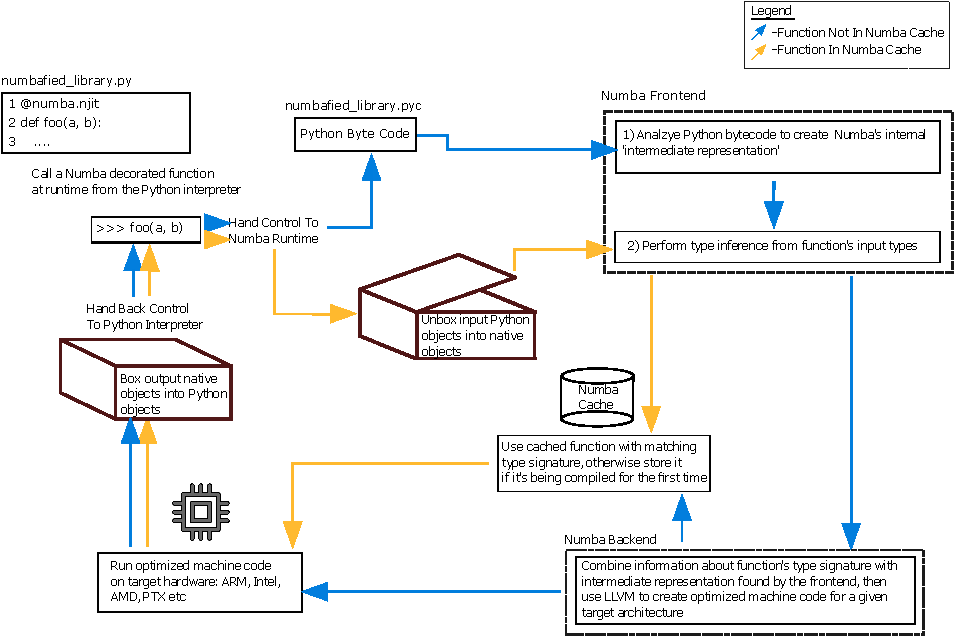
\includegraphics[width=\linewidth]{images/ch_1/numba.pdf}
    \caption{A visualisation of the Numba runtime system. A function decorated with `njit' acts as an instruction to the runtime to check a database for any Numba-compiled functions with a matching function signature, if this doesn't exist Numba generates a new compiled function and caches it using LLVM. Future calls of this function use this cached version in place of the Python interpreter. Code relies on Numba's runtime to correctly `box' and `unbox' native Python objects into data structures compatible with Numba code, which operates on a subset of numerical data structures created using the NumPy library. Figure adapted from \cite{kailasa2022pyexafmm}.}
    \label{fig:chpt:1:sec:1:numba_runtime}
\end{figure}


\pagebreak

% \begin{figure}[H]
\begin{lstlisting}[language=Python, caption={Three ways of writing a trivial algorithm in Numba, that performs some computation and saves the results to a dictionary. Adapted from Listing 2 in \cite{kailasa2022pyexafmm}},  label=code:chpt:1:sec:1:numba_compiler_optimisations]
import numpy as np
import numba
import numba.core
import numba.typed

# Initialise in the Python interpreter
data = numba.typed.Dict.empty(
    key_type=numba.core.types.unicode_type,
    value_type=numba.core.types.float64[:]
)

data['initial'] = np.ones(N)

# Subroutine 1
@numba.njit
def step_1(data):
    """
    Initialise a matrix and perform a matrix matrix product,
    storing a single column in the data dictionary.
    """
    a = np.random.rand(N, N)
    data['a'] = (a @ a)[0,:]


# Subroutine 2
@numba.njit
def step_2(data):
    """
    Initialise a matrix and perform a matrix matrix product,
    storing a single column in the data dictionary.
    """
    b = np.random.rand(N, N)
    data['b'] = (b @ b)[0,:]


@numba.njit
def algorithm_1(data):
    """
    First implementation.
    """
    step_1(data)
    step_2(data)


@numba.njit
def algorithm_2(data):
    """
    Second implementation.
    """
    # This time the storage dictionary is created within the
    # Numba function, so the types are inferred by the Numba
    # runtime, this also avoids a boxing cost to create a Numba
    # type from a Python one.
    data = dict()
    data['initial'] = np.ones(N)
    step_1(data)
    step_2(data)
    return data

@numba.njit
def algorithm_3(data):
    """
    Third implementation.
    """

    # This time, the subroutines are manually inlined
    # by the implementer, as well as the initialisation
    # of the results dictionary locally, as in algorithm_2.

    data = dict()
    data['initial'] = np.ones(N)

    def step_1(data):
        a = np.random.rand(N, N)
        data['a'] = (a @ a)[0,:]


    # Subroutine 2
    @numba.njit
    def step_2(data):
        b = np.random.rand(N, N)
        data['b'] = (b @ b)[0,:]

    step_1(data)
    step_2(data)
    return data
\end{lstlisting}
% \end{figure}
% \afterpage{\clearpage}


\begin{table}
    \centering
    \caption{Performance of different algorithms from Listing \ref{code:chpt:1:sec:1:numba_compiler_optimisations}, taken on an i7 CPU and averaged over seven runs for statistics.}
    \begin{tabular}{l l l}
        \toprule
        Algorithm & Matrix dimension & Time ($\mu s$) \\
        \midrule
        1 & \(\mathbb{R}^{1 \times 1}\) & 1.55 $\pm$ 0.01 \\
        1 & \(\mathbb{R}^{100 \times 100}\) & $304 \pm 3$\\
        1 & \(\mathbb{R}^{1000 \times 1000}\) & $29,100 \pm 234$ \\
        \midrule
        1 & \(\mathbb{R}^{1 \times 1}\) & $2.73 \pm 0.01$ \\
        1 & \(\mathbb{R}^{100 \times 100}\) & $312 \pm 3$ \\
        1 & \(\mathbb{R}^{1000 \times 1000}\) & $25,700 \pm 92$ \\
        \midrule
        1 & \(\mathbb{R}^{1 \times 1}\) & $2.71 \pm 0.01$ \\
        1 & \(\mathbb{R}^{100 \times 100}\) & $312 \pm 1$ \\
        1 & \(\mathbb{R}^{1000 \times 1000}\) & $25,700 \pm 140$ \\
        \bottomrule
    \end{tabular}
    \label{table:chpt:1:sec:1:numba_compiler_optimisations}
\end{table}

\section{Introducing Rust for Scientific Software}\label{chpt:1:sec:2}

Rust is a modern system-level programming language, introduced by Mozilla in 2015 as a direct replacement for C/C++, and is bundled with features that favour safety for shared memory programming. Having identified it as a suitable candidate for our programming environment, we list a few of its key benefits in this section.

Fortran and C/C++ have have continued to dominate high-performance scientific computing applications, the main criticism of these languages for academic software is their relatively poor developer experience. C/C++ especially has significant flexibility in the compilers, documentation, build systems and package managers that developers can choose to work with, as well as support for multiple paradigms and a growing syntax. Rust stands in contrast to this with a single centrally supported runtime system, Cargo, with common standards for testing and documentation. Additionally, there is only a single Rust compiler, rustc. This inflexibility, in addition to a strongly preferred way of organising Rust code via its Traits system, makes Rust libraries significantly more uniform and readable than corresponding C++ code. Indeed installing a Rust library, or building a binary, is often as simple as running a single command from a terminal, or adding a single line to a TOML dependency file.

The lack of a uniform building and packaging standards in C/C++ means that some projects go as far as to implement a custom build system, such as the Boost library \cite{boostbuild2022github}. With the exception of Fortran, which has made recent strides to develop a standardised modern package manager and build system, inspired by Rust's Cargo \cite{fpm2022github}, C and C++ do not have a single officially supported package manager or build system. The resulting landscape is a multitude of package managers \cite{spack2022github, vcpkg2022github, conan2022github} and build systems \cite{meson2022github, bazel2022github, scons2022github} a few of which we have cited here, all of which replicate each others functionality, none of which are universally accepted or implemented across projects nor officially supported by the C++ software foundation. Figure (\ref{fig:chpt:1:sec:2:builds}) provides an overview of a few of the myriad approaches taken in other languages. To manage this complexity, builds are often defined using a metabuild system, most commonly CMake. CMake is a scripting language, and as a meta build system it takes a specification of local and third party dependencies and hardware targets, and generates Makefiles. CMake gives developers a great deal of flexibility, it is multi-platform, and language agnostic, however it is not straightforward to maintain projects as the number of dependencies grows. Indeed, there is a significant body of literature discussing best practices with CMake \cite{scott2018professional}. However, CMake is not responsible for downloading and installing third party packages or verifying their relative compatibility, implementing its best practices is again left to users. Cargo's relative simplicity mirrors the simple build systems of high-level languages such as Python or Julia, and removes one of the main causes of development pain when working with compiled languages, and makes it significantly easier for small teams to publish software that can be easily deployed by downstream users regardless of their system's architecture or operating system.

A unique feature of Rust is its approach to ensure safe shared memory programming, enforced by its compile time `borrow checker'. Every reference in Rust has an associated `lifetime' defined by its scope, and a singular `owner'. Which enforce the programming pattern of `resource allocation is initialisation' (RAII). The basic rule is that references are owned within a scope, and dropped when out of scope. The borrow checker enforces this at compile-time, in a multithreaded context this makes it impossible to have a compiled Rust binary that has dangling pointers or double-free errors. For mutable data, the borrow checker ensures that there is only a single mutable reference at any given time in the program's runtime, ensuring that there can never be a race condition in compiled Rust code. Identifying pointer-related bugs is one of the main challenges in multi-threaded programming, with safe `smart pointers' being optional in C++, implementing RAII is left to developers.

Rust is `multi-paradigm', supporting both object oriented, and functional styles of programming. Method calls are often chained, in a functional-like style, however users can still implement methods on structs as in other object oriented languages. The unique feature introduced by Rust is its Traits system, for specifying shared behaviour, that supersedes object-oriented design. Traits are a similar to C++ 20's interfaces, in that they provide a way to enforce behaviour, rather than embedding it into a type as with traditional inheritance. However unlike C++, Rust Traits allow you to write blanket implementations, and implement interfaces for types you didn't define in your own code making them significantly more powerful. This means that behaviour can be built `bottom up', rather than `top down' as with object orientation, making it much easier for readers to identify the expected behaviour of a given Rust type by simply reading which Traits it implements. In a scientific context we are usually concerned with the organisation, reading and writing of data, commonly adhering to a design philosophy known to as data-oriented design. Traits allow us to inject additional behaviour on types without having to worry about potentially complex inheritance hierarchies.

Rust's runtime includes a test runner, a documentation generator, and a code formatter. As with other Rust features, these are maintained in lock step with the language specification, and with reference to other Rust developments. This imposes universal constraints on all Rust projects, allowing for objectively defined `good' Rust code, rather than relying on various standards of best practices that vary between projects and organisations. Furthermore the Rust compiler is highly informative, providing hints to developers on best practices for their code, as well as potential sources of bugs or code rot, by notifying users of common anti-patterns or unused variables and functions.

Despite being a young language, Rust already supports a mature ecosystem of libraries for scientific computing with high-level multithreading support \cite{rayon2018github}, numerical data containers \cite{ndarray2022github}, and tools for generating interfaces to Python via its C ABI \cite{maturin2022github}. Many tools are yet to be ported into native Rust, however high quality bindings exist for core tools such as MPI \cite{rsmpi2018github}, BLAS and LAPACK \cite{blaslapackrust2022github}, with simplified build steps often requiring only a few extra lines in the dependency TOML file. The problem with interfacing with tools written in other languages is also present when building software in Rust, however Cargo offers tools to build software written in other languages and integrate it with Rust code via the `build.rs' package, which allows one to leverage existing build systems written for software written in foreign languages. This detracts from the benefits offered by Cargo as a unified package manager and build system, raising similar problems to those encountered when building software in other compiled languages. However, we observe that this remains a concern of the software's developer, who is responsible for providing build scripts for the operating systems and hardware platforms that they wish to support, and from a downstream user perspective their build process remains the same as with pure Rust packages, where the dependency is defined in their dependency TOML file. We also note that Rust is missing key tools for scientific computing, such as a code generation for GPUs, however with mounting interest in Rust from the scientific computing community this is an active area of development.


\begin{figure}
    \centerline{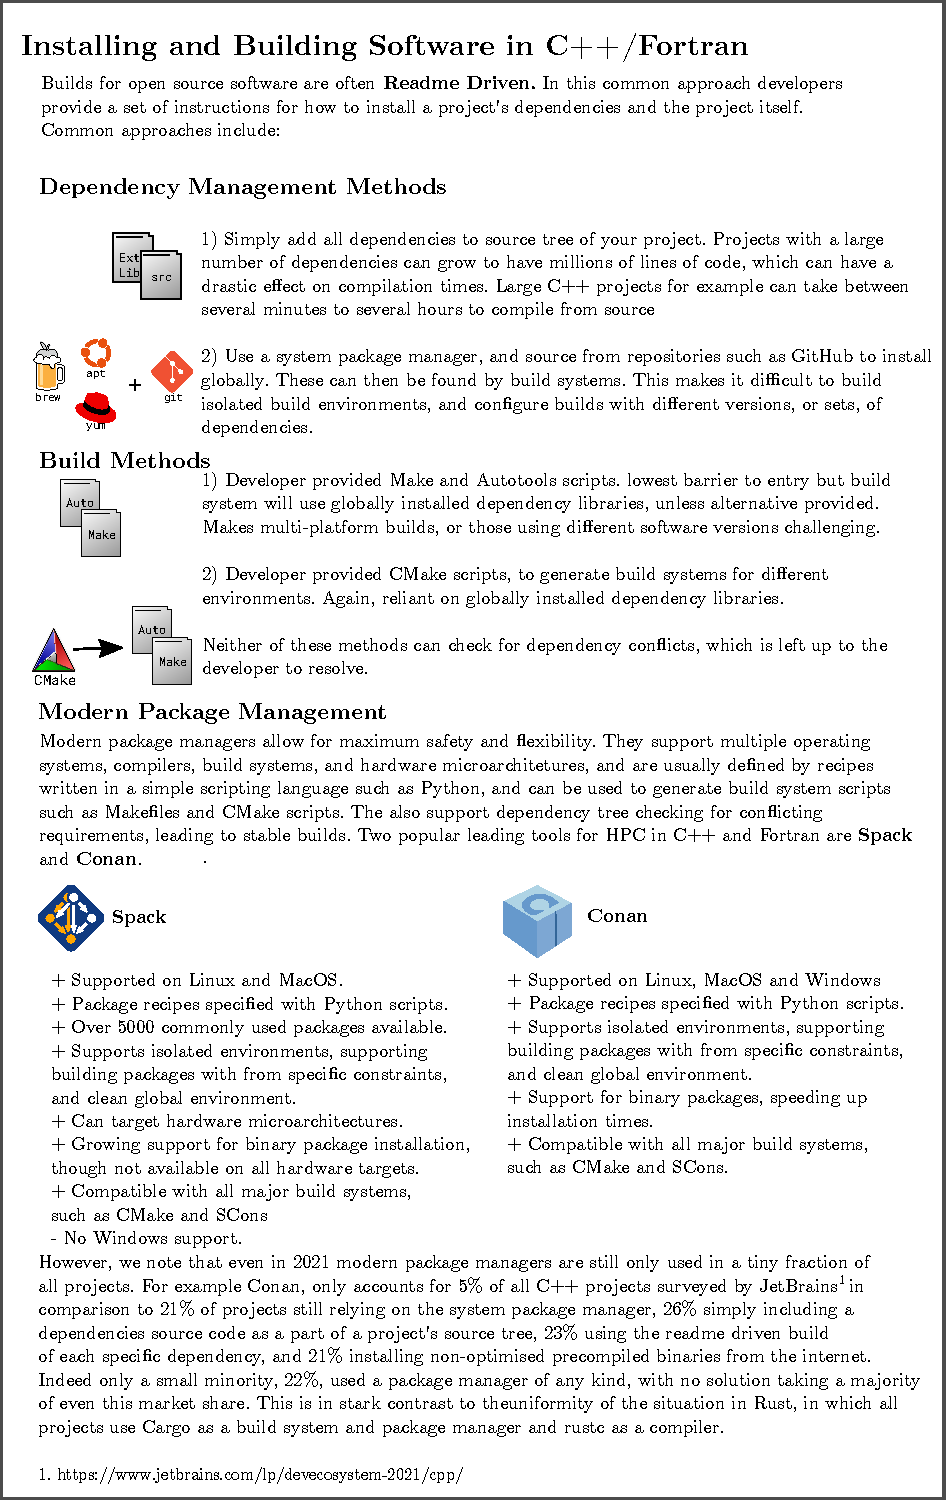
\includegraphics[width=0.95\linewidth]{ch_1/builds.pdf}}
    \caption{An overview of building software in other compiled languages.}
    \label{fig:chpt:1:sec:2:builds}
\end{figure}

\section{Future Developments}\label{chpt:1:sec:3}

Despite the above criticisms, high-level languages as tools for high-performance scientific computing remain an intense area of research and development. 'Mojo' is a new programming language, along with a compiler. It's built as a superset of Python, specifically with the two-language problem in mind. Additionally, it attempts to address the 'three language problem', whereby languages also target exotic hardware such as GPUs and TPUs \cite{Lattner2023Mojo}.

Led by a team that includes the original developers of LLVM, Mojo aims to simplify the development of high-performance applications in a Python-like language, that acts as a superset of Python. Moreover, it seeks to make these applications deployable across most hardware and software targets, ensuring compatibility with Python's vast open-source libraries and straightforward build tools.

This is achieved by building on the MLIR compiler infrastructure. MLIR can be thought of as a generalisation of LLVM, catering to CPUs, GPUs, and novel ASICs for AI. The team chose to develop around Python to leverage its extensive existing user base in computational and data sciences.

Currently, Mojo remains a closed-source language and is actively being developed by its parent company, Modular. Thus, even though it appears promising, it's not yet in a state suitable for experimentation. Nevertheless, Mojo showcases the potential of a future programming environment that might definitively `solve' the problems developers face when selecting a programming environment for academic software.
    \chapter{Designing Software for Fast Algorithms}\label{chpt:2}
Q. What is the FMM, and how does it fit into an ecosystem of Fast Algorithms?

    - Introduce the algorithmic intuition for the FMM very briefly.
        - Dump the algorithm in the appendix.
    - Zoo of FMMs/Hierarchical algorithms that have similar algorithm structure.
    - Utility relies on problem context.
        - Where some FMMs are preferable to others.
        - This makes a generic software hard \dots
    - Some FMMs are amenable to generic implementation that target a wide-class
    of problems, black box.
        - KiFMM
            - How does it create multipole and local expansions - MFS.
                - Dump MFS further explanation in the appendix.
            - How does it compute the translation operators?
                - turn it into a least squares problem
        - bbFMM
            - How does it create multipole and local expansions? Cheb.
            - How does it compute translation?
                - Not sure, need to check.

Q. What are the main challenges associated with developing bbFMMs?

    - Performant multipole to local translations. Which in bbFMMs are a matvec.
        - Main approaches to accelerate this are SVD and FFT.
        - How do these work, roughly?
            - Dump detailed explanation in the appendix.
        - Can count flops for different approaches
        - Implementation challenges
            - memory ordering for fft
            - fast ffts
            - blas3 for SVD
            - designing a generic interface for developers
            - fast trees, that can also work in dist memory
                - communication bottlenecks, and potential approaches

        - dump all algorithms into appendix

Q. What about other fast algorithms, do they require any of the same stuff used
in the FMM? What are the key areas to make generic as an implementer, has this
been done before?

    - Inverse FMM H matrix inverses, other fast direct solver approaches all
    rely on fast trees
    - trees are actually widely used in other sci comp tasks
        - current tree software, p4est
            - why can we not just use this?
                - want cross platform builds trivial
    - want to design a hierarchy of interfaces that can be used for our application,
    but also easily plug in to other work.




\section{The Software Landscape}\label{sec:2_1}
\section{Algebraic FMM Variants}\label{chpt:2:sec:1}

In its original analytical form the applicability of the FMM is limited by the requirement for explicit multipole and local expansions, as well as a restriction to matrix vector products. Subsequent decades saw the development of `algebraic' analogues to the original algorithm. These methods are similarly based on a hierarchical partitioning, whether that be of the point data using a recursive tree as with the original FMM \cite{Ying:2004:JCP,fong2009black}, or by operating on the matrix implied by the FMM's algorithmic structure directly \cite{hackbusch1999sparse,borm2003introduction,chandrasekaran2007fast}. The latter methods are collectively known as $\mathcal{H}^2$-matrix methods. Representing the FMM operation in this way has allowed the extension of the FMM to other matrix computations, such as matrix-matrix products, as well as approximations of its inverse \cite{ambikasaran2014inverse}. Notably, many of these methods don't necessarily rely on explicit multipole/local expansions for approximating fields as in the original FMM in the previous section. Examples such as the `kernel independent FMM' (kiFMM) of Ying and co-authors instead relies on the method of fundamental solutions to approximate the fields and requires only evaluating kernel values, and is applicable to a wide range of kernels from second-order linear non-oscillatory elliptic PDEs with constant coefficients such as the Laplace equation. This approach relies on some analytic considerations, however methods also exist which are interpolatory - such as the `black box FMM' (bbFMM) of Fong and Darve \cite{fong2009black}, which similarly only relies on kernel evaluations and a Chebyshev scheme to approximate fields.

In our software we choose to implement the kiFMM of Ying and coauthors, which we explain in detail below adapting the discussion from Section 3 of \cite{Ying:2004:JCP}. This method shares advantages with other algebraic FMM methods, of generality to a large class of problems, as well as opportunities to optimise computer implementations we explore in Section \ref{chpt:2:sec:1}. This approach relies on a spatial discretisation of the problem domain via an quad/octree as in the original FMM, as well as the method of fundamental solutions (MFS) for approximating the fields from point charges/masses. This method has been demonstrated to perform well on shared memory systems \cite{wang2021exafmm}, achieve similar accuracy to the analytical variant, with relatively low pre-computation required\footnote{This depends heavily on the choice of how to sparsify $T^{M2L}$, see Section \ref{chpt:3:sec:1:m2l} for more details.}. The underlying data structure of the quad/octree has been a significant area of research and development, with established high-performance methods for their construction in shared/distributed memory environments \cite{sundar2008bottom,sundar2013hyksort,BursteddeWilcoxGhattas11}.

Consider the kernels for second-order constant coefficient non-oscillatory PDEs, such as that of the Laplace equation in (\ref{eq:chpt:2:sec:0:laplace_kernel}). Such kernels satisfy the underlying PDE everywhere except the singularity location, and are smooth away from this singularity. These problems admit a unique solution for interior/exterior Dirichlet boundary value problems. The authors of \cite{Ying:2004:JCP} rely on the smoothness and uniqueness of the Dirichlet boundary value problems as basic properties to develop their FMM formulation. The problem setting as before is the calculation of (\ref{eq:chpt:2:sec:0:fmm_problem}) for the Laplace kernel, for a set of $N$ point sources $y_i$, $i = 1...N$, which we will associated with $N$ source densities $q_i$, an target locations $y_j$, $j=1...M$. As before, the source and target locations may coincide. We use an index set $I^B_s$ and $I^B_t$ to identify the sources and targets we are considering in a particular interaction. We assume that our problem is in $\mathbb{R}^3$, however the exposition is essentially the same as in $\mathbb{R}^2$.

Assuming that we have constructed our hierarchical tree partitioning, which may be adaptive, the first step is to approximate the fields due to particles contained in each leaf box. We specify more concretely that for a given box, $B$, its `near field range', $\mathcal{N}^B$, is the set of 27 boxes at the same level of a tree which are adjacent to it, i.e. they share a corner, face or edge as well as $B$ itself. Its `far field range', $\mathcal{F}^B$, is simply the boxes which are the complement of this.

We approximate the potential in $\mathcal{F}^B$ from the source densities $\{ q_i : i \in B \}$ in $B$ using the potential from an \textit{equivalent density distribution}, $q^{B, u}$, supported at prescribed locations $y^{B, u}$ (see the left box in Figure \ref{fig:chpt:2:sec:1:multipole_local}). Where $q^{B, u}$ is called the \textit{upward equivalent density} and $y^{B, u}$ is called the \textit{upward equivalent surface}. This amounts to representing the potential with a `single layer' potential \cite{Kress2014},

\begin{flalign}\label{eq:chpt:2:sec:1:single_layer_potential}
    \phi(x) &:= \int_{y \in y^{B, u}} K(x, y)q^{B, u}(y) ds(y), \> \> x \in \mathbb{R}^3 \setminus y^{B, u}
\end{flalign}

To guarantee the smoothness of the potential produced by $q^{B, u}$ in the far-field, its support $y^{B,u}$ must not overlap with $\mathcal{F}^B$ due to the singularities in this integral from the kernel function when evaluated on the equivalent surface. Secondly, we note that the equivalent surface must enclose $B$ from the definition of the single layer potential \cite{Kress2014}. We see that the equivalent surface must be placed in between the box and the boundary of $\mathcal{F}^B$.

The potential induced by our equivalent densities and upward equivalent surface satisfies the Laplace equation. Therefore, due to the uniqueness of the exterior Dirichlet boundary value problem for this kernel (as well of kernels of a similar type), we reason that the potential calculated using (\ref{eq:chpt:2:sec:0:fmm_problem}) directly from the source particles must be equivalent to that calculated using (\ref{eq:chpt:2:sec:1:single_layer_potential}) in $\mathcal{F}^B$, or anywhere between $y^{B, u}$ and $\mathcal{F}^B$. Thus we place an intermediate surface called the \textit{upward check surface} between $\mathcal{F}^B$ and $y^{B, u}$, denoting it with $x^{B, u}$. The potential computed at this surface is called the \textit{upward check potential}, which we denote by $\phi^{B, u}$.

We write this as,

\begin{flalign}\label{eq:chpt:2:sec:1:multipole_appx}
    \int_{y^{B, u}} K(x, y) q^{B, u} dy = \sum_{i \in I^B_s} K(x, y_i)q_i = \phi^{B, u}(x)\> \>, \text{for any } x \in x^{B, u}
\end{flalign}

Solving for the equivalent densities is an equivalent method of approximating the far-field potential induced by the points in $B$. We identify this with a \textit{multipole expansion}. Now considering source densities which are not contained in a box $B$ (see right box of Figure \ref{fig:chpt:2:sec:1:multipole_local}) but in its $\mathcal{F}^B$, we can construct an equivalence for local expansions using a similar approach. To ensure the existence of the \textit{downward equivalent densities} $q^{B, d}$, the \textit{downward equivalent surface}, $y^{B, d}$, must be located between $B$ and $\mathcal{F}^B$ and the potentials generated by the source points are matched to those generated by the equivalent points on a \textit{downward check surface}, $x^{B, d}$ that encloses the box and is itself enclosed by $y^{B, d}$ in order to calculate a \textit{downward check potential} $\phi^{B, d}$.

\begin{flalign}\label{eq:chpt:2:sec:1:local_appx}
    \int_{y^{B, d}} K(x, y) q^{B, d} dy = \sum_{i \in I^{\mathcal{F}^B}_s} K(x, y_i)q_i = \phi^{B, d}(x) \> \> \text{for any } x \in x^{B, d}
\end{flalign}

In $\mathbb{R}^3$ the authors chose to represent the equivalent and check surfaces as cubes, with the equivalent/check points arranged regularly over the surfaces. We choose the same as it leads to implementation benefits when designing the field translation operators (see Section \ref{chpt:3:sec:1:subsec:2:fft} for how we take advantage of this).

\begin{figure}
    \centering
    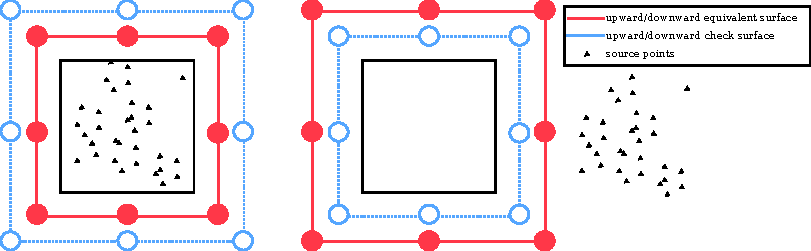
\includegraphics[width=\textwidth]{ch_2/p2m.pdf}
    \caption{ We illustrate the equivalent/check surfaces and associated boxes in $\mathbb{R}^3$, where we show a corresponding cross section. In the first figure, we illustrate the situation in the `P2M' operation, where we are trying to construct an approximation to the potential generated by points in a box by matching it to that generated by a set of equivalent density points placed on a fictitious surface enclosing it. In the second figure we illustrate the `P2L' operation, where we are now trying to construct an approximation to the  potential generated by points in a box's far-field within the box.}
    \label{fig:chpt:2:sec:1:multipole_local}
\end{figure}

Equations (\ref{eq:chpt:2:sec:1:multipole_appx}) and (\ref{eq:chpt:2:sec:1:local_appx}) are examples of \textit{Fredholm integral equations of the first kind}, the inversion of which is ill-posed. To solve these equations, we must first discretise, for which we made use of the \textit{Method of Fundamental Solutions} (MFS), a technique whereby the potential is approximated by a linear combination of kernel function evaluations at a set of discrete points with associated densities,

\begin{flalign}\label{eq:chpt:2:sec:1:mfs}
    \phi(x) \approx \phi^N(x) = \sum_{y_i \in y^{B, u}} K(x, y_i) q_i
\end{flalign}

Where $N$ denotes the number of equivalent points of density are placed on the equivalent surface. To see how this approximates the single-layer operator we used above to calculate the potential we simply replace the continuous density functions in (\ref{eq:chpt:2:sec:1:single_layer_potential}) with $\sum_{j=1}^N q_i \delta(y-y_j)$, recovering (\ref{eq:chpt:2:sec:1:mfs}). Writing (\ref{eq:chpt:2:sec:1:multipole_appx}) or (\ref{eq:chpt:2:sec:1:local_appx}) in matrix form reflecting the discretisation via MFS,

\begin{flalign}
    K q = \phi
\end{flalign}

We can solve the problem with Tikhonov regularisation,

\begin{flalign}
    q = (\alpha I + K^* K)^{-1}K^*\phi
\end{flalign}

which converts it into a matrix equation, that shares similarities in terms of well posedness with discretised \textit{Fredholm integral equations of the second kind}. The regularisation parameter $\alpha$ is found empirically. Computing (\ref{eq:chpt:2:sec:1:multipole_appx}) is equivalent to the $T^{P2M}$ operator described in the previous section for the analytical FMM, (\ref{eq:chpt:2:sec:1:local_appx}) is equivalent to an $T^{P2L}$ operator which was not explicitly described. As before, these operators take a set of charges, and create expansions that allow us to evaluate their potential in the far-field, however the method of creating the expansions is clearly significantly different. The most notable change being that our above formulation \textit{does not require explicit analytical expansions of the kernel function}, only making use of kernel evaluations.

To complete the kiFMM we need analogues to the field translation operators, $T^{M2L}$, $T^{M2M}$, $T^{L2L}$. We illustrate the required surfaces for each of these operators in Figure \ref{fig:chpt:2:sec:1:translations}. For $T^{M2M}$ we must translate the upward equivalent density of $A$ to the centre of its parent box $B$, solving the following equation for $q^{B, u}$,

\begin{flalign}
    \label{eq:chpt:2:sec:1:m2m}
    \int_{y^{B, u}} K(x, y)q^{B, u}(y)dy = \int_{y^{A, u}}K(x, y)q^{A, u}(y) dy, \> \> \text{for all } x \in x^{B, u}
\end{flalign}

As before, $y^{A, u}$ must enclose the child box $A$. During the downward pass, we must evaluate the downward equivalent density, corresponding to a local expansion, from the multipole expansions of non-adjacent boxes in $B$'s parent neighbour's children. We similarly write down for $T^{M2L}$,

\begin{flalign}
    \label{eq:chpt:2:sec:1:m2l}
    \int_{y^{B, d}} K(x, y)q^{B, d}(y)dy = \int_{y^{A, u}}K(x, y)q^{A, u}(y) dy, \> \> \text{for all } x \in x^{B, d}
\end{flalign}

Finally, the local expansions of each box $B$ must be translated to the centre of each of its children $A$,

\begin{flalign}
    \label{eq:chpt:2:sec:1:l2l}
    \int_{y^{B, d}} K(x, y)q^{B, d}(y)dy = \int_{y^{A, d}}K(x, y)q^{A, d}(y) dy, \> \> \text{for all } x \in x^{B, d}
\end{flalign}

For each of these translation operators we use the discretisation based on MFS discussed above, and solve using Tikhonov regularisation. For the  $T^{L2P}$, $P2P$ and $T^{M2P}$ operators we simply use direct kernel evaluations at the target points with respect to the equivalent densities represented by the multipole or local expansion coefficients or the true densities at the source points.

\begin{figure}
    \centering
    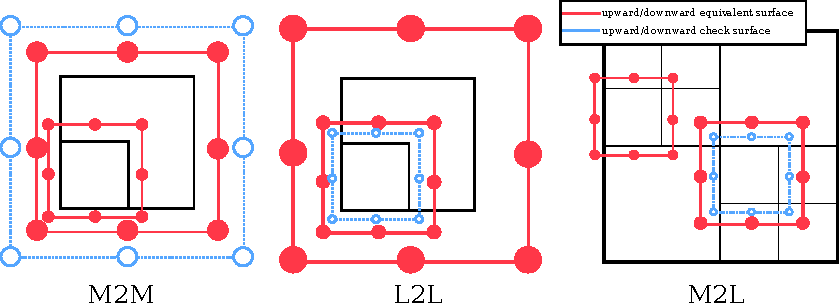
\includegraphics[width=\textwidth]{ch_2/translations.pdf}
    \caption{ As in Figure \ref{fig:chpt:2:sec:1:multipole_local}, we illustrate the translations as cross sections of the surfaces, which are cubes in $\mathbb{R}^3$.}
    \label{fig:chpt:2:sec:1:translations}
\end{figure}



\section{Case Study: PyExaFMM, a Python FMM}\label{sec:2_2}
\section{Implementation Challenges for the Kernel Independent Fast Multipole Method }\label{chpt:2:sec:2}

In this section we introduce analytical features of the kernels compatible with the kiFMM that have consequences for computer implementations, such as the ability to pre-compute and cache matrices that correspond to translation operators. We also discuss the octree data structure in more detail, highlighting its key bottlenecks, concluding with a discussion on implied computational and storage complexity.

The defining feature of the kernels compatible with the FMM is that they they display a rapid decay behaviour as the distance between interactions increases, known formally as \textit{asymptotic smoothness}. A kernel is described as asymptotically smooth if there are constants $C_{\text{as1}}, C_{\text{as2}} \in \mathbb{R}_{>0}$ that satisfy \cite{borm2003introduction},

\begin{flalign}
        \label{eq:chpt:2:sec:1:asym_smooth}
    | \partial_x^\alpha \partial_y^\beta K(x, y) | \leq C_{\text{as1}} (C_{\text{as2}} \|| x-y \|_2)^{-|a|-|b|}\alpha + \beta|K(x, y)|
\end{flalign}

for all multi-indices $\alpha, \beta \in \mathbb{N}^3_0$ and all $x, y \in \mathbb{R}^3$. It's this smoothness that allows us to limit the definition of $\mathcal{N}^B$ to its neighbouring boxes in the FMM. Considering the situation in $\mathbb{R}^3$ only, this leads to $|\mathcal{N}^B| = 3^3=27$.

Far-field interactions are handled by the $T^{M2L}$ step, we saw above how this is limited to interactions with boxes which are children of $B$'s parent, but non-adjacent to $B$. Therefore we see that in a multi-level scheme the $\mathcal{N}^B$ contains all of the $6^3=216$ near and far field interactions of $B$'s children. As far-field interactions necessarily exclude the near field, this leads to a maximum of $6^3-3^3=189$ boxes in each child box's far field that must be considered, each corresponding to a single $T^{M2L}$. This is one of the \textit{key bottlenecks} of efficient FMM implementations. There are numerous ways of \textit{sparsifying} this step, either by using some additional numerical technique such as an SVD to compress the matrices corresponding to $T^{M2L}$ as they are known to be low-rank, or by using an exact method such as an Fast Fourier Transform (FFT) - which relies on our decision to place the equivalent densities on a regular grid as then the $T^{M2L}$ can be re-interpreted as a convolution. We discuss the trade-offs of these approaches in detail in Section \ref{chpt:3:sec:1:m2l}, as optimal implementations of this sparsification are of central importance to our software's performance.

We note that precomputations can be further reduced if kernels also exhibit translational invariance,

\begin{flalign}
    \label{eq:chpt:2:sec:1:translational_invariance}
    K(x, y) = K(x+v, y+v)
\end{flalign}

where $v \in \mathbb{R}^3$, we can compute $T^{M2L}$ for a restricted subset of the total possible interactions for the eight child boxes. Indeed, the union of all possible far-field interactions for the eight child boxes gives $7^3-3^3 = 316$ possible interactions. This comes from the fact some subset of translation vectors are non-overlapping for each child, resulting in a total of $7^3$ total interactions for all children, subtracting the near-field interactions which are the same for all children gives the result. Furthermore this means that we must pre-compute just 316 unique $T^{M2L}$ if our kernel has these favourable properties. This is of course dependent on choosing the same equivalent and check surfaces, and density locations, for each box. If so, these can be pre-computed and cached for a given expansion order, corresponding to all possible $T^{M2L}$ at each level.

If an asymptotically smooth, translationally invariant, kernel is also homogeneous to degree $n$,

\begin{flalign}
    K(\alpha r) = \alpha^n K(r)
\end{flalign}

where $\alpha \in \mathbb{R}$, implies that when we scale the distance between a source and target box by $\alpha$ the potential is scaled by a factor of $\alpha^n$, where $n$ depends on the kernel function in question, we can compute $T^{M2L}$ for a \textit{single} level of the tree, and scale the result at subsequent levels. This is summarised in Table \ref{table:chpt:2:sec:1:m2l_optimisations}.

\begin{table}
    \centering
    \caption{Number of near and far field boxes for a given box $B$, depending on the type of kernel we're considering.}
    \begin{tabular}{l l l}
        \toprule
        Kernel Type & boxes in $\mathcal{N}^B$ & boxes in $\mathcal{F}^B$ \\
        \midrule
        trans. invar. & $\leq$ 27 per box & $\leq$ 316 per level \\
        trans. invar. + homog. & $\leq$ 27 per box & $\leq$ 316 in total\\
        \bottomrule
    \end{tabular}
    \label{table:chpt:2:sec:1:m2l_optimisations}
\end{table}

As we've chosen the location of point densities to be fixed relative to each box, the evaluation of (\ref{eq:chpt:2:sec:1:m2m}) and (\ref{eq:chpt:2:sec:1:l2l}) can equivalently be pre-computed. In this case, there are just 8 unique matrices corresponding to $T^{M2M}$ and $T^{L2L}$, corresponding to the relative positions between a parent box and its children.

We observe the $T^{P2M}$ is calculated for all the nodes of a quad/octree in a discretisation, as observed in the previous section the level of discretisation is either specified by the user, or set by a user defined constraint $N_{\text{crit}}$ which specifies a maximum number of points contained within each leaf box. This leads to $O(N \cdot N_{\text{crit}})$ to find the check potentials for each leaf, therefore we note that $N_{\text{crit}}$ must be kept small to ensure linear complexity is maintained for this operation. To compute the equivalent density, we rely on an application of the inverted integral operator in (\ref{eq:chpt:2:sec:1:multipole_appx}). The size of this matrix is determined by the expansion order $P$, which determines the number of quadrature points taken on the equivalent/check surfaces. As the points are taken to be placed on a regular grid over this surface, the number of quadrature points $N_{\text{quad}}$ relates to $P$ as,

\begin{flalign}\label{eq:chpt:2:sec:2:ncoeffs}
    N_{\text{quad}} = 6(P-1)^2+2
\end{flalign}

Therefore, this matrix vector product is of $O((P-1)^4)$, leading to $O(N((P-1)^4 + N_{\text{crit}}))$ complexity for the entire operator. The complexity of $T^{P2L}$ is the same, as it amounts to the same calculation, albeit to form a local expansion. The precomputation of the translation operator requires an SVD for the integral operator in (\ref{eq:chpt:2:sec:1:multipole_appx}), the complexity of which is dependent on the algorithm chosen, with implementation specific optimisations. However, for a $\mathbb{R}^{m \times n}$ matrix where $m$ and $n$ are of similar size, the `DGESVD' implementation of LAPACK, which we use in our software framework, has a complexity of $O(n^3)$ therefore this precomputation is of $O((P-1)^6)$. The storage required is of $O((P-1)^4)$ for the inverted matrix.

Applying similar analysis for computing (\ref{eq:chpt:2:sec:1:m2m}) and (\ref{eq:chpt:2:sec:1:l2l}), we arrive at computational complexities of $O(N \cdot (P-1)^4)$ for calculating the check potentials, and then evaluating the equivalent densities via two matrix-vector products. For the M2L step, if we do not choose to implement any sparsification, we also obtain $O(N \cdot (P-1)^4)$ for the asymptotic complexity of applying $T^{M2L}$, however here there are large lurking constants. Specifically, each box $B$ has to apply an $T^{M2L}$ up to 189 times in $\mathbb{R}^3$ or 27 times in $\mathbb{R}^2$. The storage complexity is determined by the kernel, as shown by table \ref{table:chpt:2:sec:1:m2l_optimisations}, the properties of the kernel can reduce the number of precomputations that can be cached.

Similar large constants lurk in the leaf level computations $P2P$, $T^{M2P}$, $T^{P2L}$. These all consider boxes contained in $B$'s near field. For non-uniform point distribution there could be very large number of boxes contained in the near field. Therefore to reduce this we enforce a `balancing' condition, as mentioned above. The most common condition is a `2:1 balance', whereby neighbouring boxes are restricted to be no more than twice as large as each other \cite{malhotra2015pvfmm}. This restricts the size of the number of adjacent boxes to $B$ to be at most 52 in $\mathbb{R}^3$. For these boxes we will calculate the potential for points in $B$ using kernel evaluations directly via $P2P$. For the remainder of its near field, we'll use the $T^{M2P}$ operator. This operator considers boxes in $B$' near field for which the multipole expansion still applies at $B$, this means that leaf boxes that coincide with $B$'s neighbours children that are non-adjacent to $B$. At most there are 156 such boxes in $\mathbb{R}^3$. There may also be an additional contribution to the local expansion at $B$ not captured in $T^{L2L}$ and $T^{M2L}$, from boxes in the near-field of $B$'s parent which are the leaf level, and considered in the far-field of $B$ itself, and are the level of $B$'s parent. These contributions are found via $T^{P2L}$. With our balancing condition there are at most 19 such boxes in $\mathbb{R}^3$. We note that for uniformly refined trees $T^{M2P}$ and $T^{P2L}$ aren't calculated as their corresponding interactions are subsumed into $P2P$. The $P2P$ operator is therefore of $O(52 N \cdot N_{\text{crit}})$, with no storage cost as this is applied directly to points. Similarly, the complexity of $T^{M2P}$ is $O(156 N \cdot (P-1)^2 N_\text{crit})$, $T^{L2P}$ is of $O(N (P-1)^2 \cdot N_\text{crit})$. The complexity of $T^{P2L}$ is $O(19 N \cdot ((P-1)^4 + N_\text{crit}))$, where we include the cost of calculating the check potential as in $T^{P2M}$. The complexities of each step are summarised in table \ref{table:chpt:2:sec:2:kifmm_complexities}. These complexities are only an upper bound, for $T^{M2P}$ and $T^{P2L}$, and correspond to quite extreme point distributions, rarely occuring for all boxes in a given discretisation. In practice these are found to be an order of magnitude smaller than the number of boxes that must be considered in $T^{M2L}$ for point distributions that are relatively uniform \footnote{For example for randomly distributed on the surface of a sphere, or normally distributed points, typical values are $O(10)$ boxes for $T^{M2P}$ and $O(1)$ boxes for $T^{L2P}$}.

Therefore the largest bottlenecks are the $P2P$ and $T^{M2L}$ steps, and the area of focus in optimised implementations. When implemented naively, $T^{M2L}$ contains a large number of BLAS level 2 operations, and is calculated for every non-leaf box below the first level of an octree/quadtree. An obvious optimisation is to re-order data such that a single BLAS level 3 operation is computed for each box. This increases the ratio of computations to memory accesses by converting a series of matrix-vectors product into a single matrix-matrix product for each box. Additionally, the SVD taken for the integral operators above can be cut-off due to the low-rank nature of the above operators, leading to a reduced storage and application complexity. We explore the rank behaviour in more detail in Chapter \ref{chpt:3:sec:1:m2l} for the Laplace kernel. If instead one chooses to take an FFT, which offers lower complexity for each $T^{M2L}$ while being an exact translation, one has to compute the FFT corresponding to each unique translation which as we've seen is kernel dependent, and perform an inverse FFT to evaluate the check potentials at the equivalent density points. This leads to a lower overall complexity for both compute and storage - however, as we observe in Section \ref{chpt:3:sec:1:subsec:2:fft}, memory accesses are critical to performant implementations. The performance of the $P2P$, $T^{M2P}$ and $T^{L2P}$ operators are determined most significantly by the ability to rapidly evaluate the kernel function over sets of points. This is a ripe area for compute optimisations, such as GPU off-loading, or developing vectorised CPU code, and is therefore highly-dependent on the available computational resources and their respective architectures. Practical implementations should be flexible enough to for developers to `plug-in' different implementations in order to experiment with new hardware.

The second major bottleneck with the kiFMM and FMMs more generally, especially in a distributed setting, is the quad/octree data structure. The tree is crucial to performance as being able to rapidly query, and communicate via the tree, especially in a distributed setting will determine the overall runtime, as communication latency is a leading order variable in the distributed FMM's complexity \cite{Yokota2014}. Though there has been significant scholarship in developing high-performance tree libraries for parallel and distributed settings \cite{BursteddeWilcoxGhattas11,sundar2008bottom,sundar2013hyksort}, we observe that relatively little work has been done to examine and develop tree libraries with the FMM explicitly in mind, we explore potential optimisations in Section \ref{chpt:3:sec:0:octrees}. Specifically, $T^{M2M}$ summarises global information that is required by each box, and is later distributed via $T^{M2L}$ this necessarily involve communication across node boundaries in a distributed setting. Additionally, the broad applicability of parallel trees necessitates a design of software that is relatively de-coupled from the FMM code to encourage adoption in other communities. These two concerns determine the implementation strategy of our own tree library.

\begin{table}
    \centering
    \caption{Asmyptotic complexities of each kiFMM operator in $\mathbb{R}^3$, with constants left to demonstrate relative contrast. For $T^{M2L}$ we provide a few different complexity estimates, starting with `naive' implementation which applies the inverted integral equation (\ref{eq:chpt:2:sec:1:m2l}) up to 189 for each box as a matrix vector product, with no sparsification. Then the complexities with respect to different kernel properties. For an $T^{M2L}$ sparsified via the SVD we indicate a cut-off rank with $\kappa$, for an FFT based approach as we are often working with real data for the densities we can retain only half the calculated frequencies to save on storage costs. For the $T^{P2L}$, $T^{M2P}$ and $P2P$ operators we provide estimates for 2:1 balanced trees, as we restrict ourselves to this a practical implementation.}
    \begin{tabular}{l l l}
        \toprule
        Operator & Computational Complexity & Storage Complexity  \\
        \midrule
        $T^{P2M}$ & $O(N(36(P-1)^4 + N_{\text{crit}}))$ & $O(36(P-1)^4)$\\
        \midrule
        $T^{M2M}$ & $O(36N(P-1)^4)$ & $O(8 \cdot 36(P-1)^4)$\\
        \midrule
        $T^{L2L}$ & $O(36N(P-1)^4)$ & $O(8 \cdot 36(P-1)^4)$\\
        \midrule
        $T^{M2L}_\text{naive}$ & $O(189N \cdot 36(P-1)^4)$ & $O(189N \cdot 36(P-1)^4)$ \\
        \midrule
        $T^{M2L}_\text{trans. inv.}$ & $O(189N \cdot 36(P-1)^4)$ & $O(316 \log(N) \cdot 36(P-1)^4)$ \\
        \midrule
        $T^{M2L}_\text{homog+trans. inv.}$ & $O(189N \cdot 36(P-1)^4)$ & $O(316 \cdot 36(P-1)^4)$ \\
        \midrule
        $T^{M2L}_\text{homog+trans. inv. + SVD}$ & $O(189N \cdot 6(P-1)^2 \cdot \kappa )$ & $O(316 \cdot 6(P-1)^2 \cdot \kappa)$ \\
        \midrule
        $T^{M2L}_\text{homog+trans. inv. + FFT}$ & $O(189N \cdot 4 (P-1) \log(P-1))$ & $O(316 \cdot 36(P-1)^4)$ \\
        \midrule
    $T^{M2L}_\text{homog+trans. inv. + Real FFT}$ & $O(189 N \cdot 4 (P-1) \log(P-1))$ & $O(316 \cdot 18(P-1)^4)$ \\
        \midrule
        $T^{L2P}$ & $O(N(36(P-1)^4 + N_{\text{crit}}))$ & $O(1)$\\
        \midrule
        $T^{P2L}_\text{balanced}$ & $O(19 N \cdot (36(P-1)^4 + N_{\text{crit}}))$ & $O(1)$\\
        \midrule
        $T^{M2P}_\text{balanced}$ & $O(156 N \cdot ( 36(P-1)^4) )$ & $O(1)$\\
        \midrule
        $P2P_\text{balanced}$ & $O(52 N \cdot N_\text{crit} )$ & $O(1)$ \\
        \bottomrule
    \end{tabular}
    \label{table:chpt:2:sec:2:kifmm_complexities}
\end{table}


\section{Rust for High Performance Computing}\label{sec:2_3}
- Summary of Rust's core features for computational science.

- cargo, code organisation features, traits system, python interfacing.

- Rebuke common misconceptions: safety (bounds checking), lack of appropriate libraries for numerical data.

- Highlight what actually is missing, e.g. rust-native tools (linear algebra, MPI etc) - and what's being done about it.

- When is using rust appropriate? When is it not?

- Why are we turning to rust for this project?


\section{Case Study: RustyTree, a Rust based Parallel Octree}\label{sec:2_4}
Octrees are a foundational data structure for fast algorithms in $\mathbb{R}^3$. Writing software for octrees that can be distributed across parallel computing systems is challenging, demonstrated by the limited availability of open-source software \cite{BursteddeWilcoxGhattas11,fernando2020github}. This is inspite of their ubiquity in scientific computing applications from adaptive finite-element methods to many-body algorithms \cite{sundar2008bottom}. We present Rusty Tree, an implementation of MPI-distributed octrees with a complete Python interface. Rusty Tree is a proof of concept for Rust as a tool for high-performance computational science. We document our experience in developing Rusty Tree, and use it as a tool to explore the current landscape of scientific computing with Rust. From multithreading, and developing a Python interface, to distributing applications with MPI, writing Rusty Tree involved using much of Rust's scientific computing ecosystem. 

\subsection*{Parallel Octrees}

As mentioned in section \ref{sec:2_2}, there are multiple representations of octrees. We choose a linear octree representation, in which we discard interior nodes and store a list of leaves, as in our previous work PyExaFMM \cite{kailasa2022pyexafmm}. These lie in contrast to pointer based octrees in which each node stores pointers to its parent as well as children, which have a relatively higher storage cost, in addition to a synchronisation and communication overhead for parallel implementations that must keep track of pointers across nodes \cite{tu2005scalable}. 

Octrees are usually constructed `top down'. A user specifies a threshold for the maximum number of particles in a leaf node, $n_{\text{crit}}$, and a unit cube encapsulating the problem domain is refined until this is satisfied. After refinement, one can optionally `balance' adjacent leaf nodes such that adjacent nodes obey a relative size constraint. However, translating this logic to a parallel setting is challenging. Constructing octrees `top down' involve a significant data communication that come from having to synchronise nodes across processors during refinement. Balancing requires updating a chain of relationships, that can `ripple' across processors. Furthermore, as the data distribution is not known a priori, load balancing must be done as a post-processing step.

Sundar et al introduce `bottom up' tree construction \cite{sundar2008bottom}. The strategy relies on a `space filling curve' that passes through each octant in an octree, for which they choose a Morton encoding (see fig. (\ref{fig:sec_2_4:morton}) for a description of Morton encoding for an octant). Morton encodings have excellent properties for spatial decompositions. Once sorted, adjacent Morton keys encode spatial locality. Indeed traversing a sorted list of Morton keys from smallest to greatest is equivalent to a level by level traversal of an octree, starting at its root node. Similarly, a reverse order traversal is equivalent to a level by level traversal of an octree starting at its leaf level. This process is accelerated in RustyTree using the Rayon library for parallel multithreading which we examine in figure (\ref{fig:sec_2_4:rayon}). We build on Sundar et. al's original paper in two key ways. Firstly, we use HykSort \cite{sundar2013hyksort}, which reduces global data communication cost in comparison to a naive \pythoninline{MPIAllToAllv}, and use a combination of local balancing (alg. (\ref{alg:sec_2_4:balance_octree})) and parallel sorting \textit{avoid} their complex `ripple propagation' scheme to balance a distributed tree.

\begin{figure}
    \centerline{\includegraphics[width=\linewidth]{ch_2/morton.pdf}}
    \caption{How to Morton encode a node in an octree. [TODO: Extend graphic to explain Morton ordering]}
    \label{fig:sec_2_4:morton}
\end{figure}

Given a set of distributed point data spread across $n_p$ processors, our strategy is as follows:

\begin{enumerate}
    \item Generate a Morton key for each point corresponding to a user defined octree depth.
    \item Perform a parallel sort of these leaf octants using MPI, such that processors with adjacent MPI ranks have adjacent data.
    \item \textit{Linearise} leaves on each processor, such that their leaves do not overlap, in a manner that favours larger leaves over smaller ones, as in algorithm (\ref{alg:sec_2_4:linearise_octree}). 
    \item \textit{Complete} the space defined by the leaves on each processor, and find the domain occupied by their leaves, see figure [TODO: COMPLETE REGION] and algorithm (\ref{alg:sec_2_4:complete_region}). Define the coarsest nodes of this set as \textit{seeds}.
    \item Construct a \textit{block tree}, by completing the space between the seeds with the minimum spanning set of nodes, described in algorithm (\ref{alg:sec_2_4:complete_octree}). The nodes of this block tree are referred to as \textit{blocks}. This gives us a distributed coarse complete linear octree that is based on the underlying data distribution, and is described in algorithm.
    \item The load of each block is calculated by using the number of original octants calculated in step (1). The blocks are then redistributed so that each processor contains an approximately equal load, using algorithm (\ref{alg:sec_2_4:partition}).
    \item Point data is communicated to the processor containing its associated block, and the blocks are refined based on $n_{\text{crit}}$, providing the final, load balanced, linear octree tree.
    \item Optionally, the tree is \textit{balanced}. This can be done for the local subtree on each processor using algorithm (\ref{alg:sec_2_4:balance_octree}) The locally balanced trees can then be sorted in parallel again, and locally linearized as in step (3).
\end{enumerate}

This is summarised in algorithm (\ref{alg:sec_2_4:point2octree}). The complexity of this process is bounded by the parallel sorts, which for randomly distributed point data, run in $O(N_{\text{leaf}} \log (N_{\text{leaf}}))$ work and $O(\frac{N_{\text{leaf}}}{n_p} \log(\frac{N_{\text{leaf}}}{n_p}) + n_p \log (n_p))$ time where $N_{\text{leaf}}$ is the number of leaves in the final octree, and $n_p$ is the number of processors (see appendix \ref{app:a_2_complexity_tree_construction} for a derivation). This makes the efficiency of the parallel sort a bottleneck in tree construction.

\begin{figure}
    \centerline{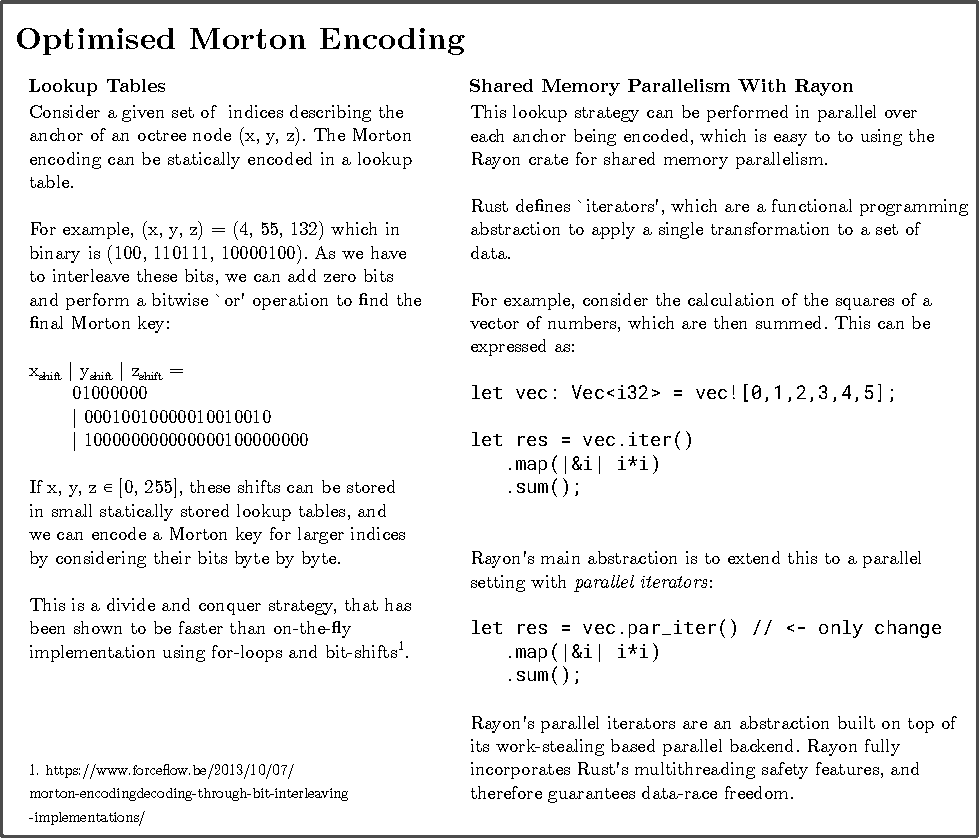
\includegraphics[width=\linewidth]{ch_2/rayon.pdf}}
    \caption{Optimising Morton encodings using shared memory parallelism and lookup tables.}
    \label{fig:sec_2_4:rayon}
\end{figure}

\begin{algorithm}
    \caption{\textbf{Remove Overlaps From Sorted List of Octants (Sequential)}: We refer to this as \textit{Linearization}.}
    \label{alg:sec_2_4:linearise_octree}
    \begin{algorithmic}
    
        \STATE \textbf{Input}: A sorted list of octants, $W$.
        \STATE \textbf{Output}: $R$, an octree with no overlaps.
        \STATE \textbf{Work}: $O(n)$, where $n$=len($W$).
        \STATE \textbf{Storage}: $O(n)$, where $n$=len($W$).
    

        \FOR{i $\gets$ 1 to len($W$)}
            \IF {$W[i] \notin \{ \text{Ancestors}(W[i+1])\}$}
                \STATE $R \gets R + W[i]$  
            \ENDIF
        \ENDFOR
        \STATE $R\gets R+W$[len($i$)]
    \end{algorithmic}
\end{algorithm}
    

\begin{algorithm}
    \caption{\textbf{Construct a Minimal Linear Octree Between Two Octants (Sequential)}: We refer to this as \textit{Completion}.}
    \label{alg:sec_2_4:complete_region}
    \begin{algorithmic}
        \STATE \textbf{Input}: Two octants $a$ and $b$, where $a > b$ in Morton order. 
        \STATE \textbf{Output}: $R$, minimal linear octree between $a$ and $b$. 
        \STATE \textbf{Work}: $O(n \log n)$, where $n$=len($R$).
        \STATE \textbf{Storage}: $O(n)$, where $n$=len($R$).

        \FOR {$w \in W$}
            \IF {$a < w < b$ \textbf{and} $w \notin \{ \text{Ancestors}(b)\}$}
                \STATE $R \gets R + w$
            \ELSIF {$w \notin \{\text{Ancestors}(a), \text{Ancestors}(b)\}$}
                \STATE $W \gets W - w + \text{Children}(w)$
            \ENDIF
        \ENDFOR
        \STATE \text{Sort}($R$)
    \end{algorithmic}
\end{algorithm}


\begin{algorithm}
    \caption{\textbf{Balance a Local Octree (Sequential)}: A 2:1 balancing is enforced, such that adjacent octants are at most twice as large as each other.}
    \label{alg:sec_2_4:balance_octree}
    \begin{algorithmic}
        \STATE \textbf{Input}: A local octree $W$, on a given node.
        \STATE \textbf{Output}: $R$, a 2:1 balanced octree. 
        \STATE \textbf{Work}: $O(n \log n)$, where $n$=len($R$).
        \STATE \textbf{Storage}: $O(n)$, where $n$=len($W$).

        \STATE $R = \text{RemoveOverlaps}(W)$
        \FOR {$l \gets \text{Depth } \text{to } {1} $}
            \STATE $Q \gets \{ x \in W | \text{Level}(x) = l \}$
            \FOR {$q \in Q$}
                \FOR {$n \in \{\text{Neighbours}(q), q\}$}
                    \IF {$n \notin R$ and $\text{Parent}(n) \notin R$}
                        \STATE $R \gets R + \text{Parent}(n)$
                        \STATE $R \gets R + \text{Siblings}(\text{Parent}(n))$
                    \ENDIF
                \ENDFOR
            \ENDFOR
        \ENDFOR
    \end{algorithmic}
\end{algorithm}


\begin{algorithm}
    \caption{\textbf{Partition a Distributed List of Octants (Parallel)}.}
    \label{alg:sec_2_4:partition}
    \begin{algorithmic}
        \STATE \textbf{Input}: A distributed list of octants, $W$. 
        \STATE \textbf{Output}: The octants redistributed across processors such that the total weight on each processor is roughly the same. 
        \STATE \textbf{Work}: $O(n)$, where $n$=len($W$).
        \STATE \textbf{Storage}: $O(n)$, where $n$=len($W$).

        \STATE $S \gets$ Scan(Weight($W$))
        \IF {rank = $n_p-1$}
            TotalWeight $\gets$ max($S$)
        \ENDIF
        \STATE $\bar{w} \gets \frac{\text{TotalWeight}}{n_p}$
        \STATE $k \gets \text{TotalWeight} \mod n_p$
        $Q_{tot} \gets \emptyset$
        \FOR { $p \gets 1$ to $n_p$}
            \IF {$p \leq k$}
                \STATE $Q \gets \{ x \in W | (p-1)(\bar{w} + 1) \leq S(x) < p (\bar{w}+1) \}$
            \ELSE
                \STATE $Q \gets \{ x \in W | (p-1)\bar{w} + k < S(x) < p \bar{w} + k \}$
            \ENDIF

            \STATE $Q_{tot} \gets Q_{tot} + Q$
        \ENDFOR
        \STATE $R \gets$ Receive()
        \STATE $W \gets W-Q_{tot}+R$
    \end{algorithmic}
\end{algorithm}

\begin{algorithm}
    \caption{\textbf{Construct a Complete Linear Octree From a Set of Seed Octants Spread Across Processors (Parallel)}}
    \label{alg:sec_2_4:complete_octree}
    \begin{algorithmic}
        \STATE \textbf{Input}: A distributed sorted list of seeds $L$.
        \STATE \textbf{Output}: $R$, a complete linear octree. 
        \STATE \textbf{Work}: $O(n \log n)$, where $n$=len($R$).
        \STATE \textbf{Storage}: $O(n)$, where $n$=len($R$).

        \STATE $R = \text{RemoveOverlaps}(L)$
        \STATE $L \gets \text{Linearise}(L)$, using algorithm (\ref{alg:sec_2_4:linearise_octree}).
        \STATE $\text{Partition}(L)$, using algorithm (\ref{alg:sec_2_4:partition}) 

        \IF {rank == 0}
            \STATE $L$.push\_front(FirstChild(FinestAncestors(DeepestFirstDescendent(root), $L$[1])))
        \ENDIF
        
        \IF {rank == $n_p-1$ }
            \STATE $L$.push\_back(LastChild(FinestAncestors(DeepestLastDescendent(root), $L$[len($L$)])))
        \ENDIF

        \IF {rank > 0}
            \STATE Send($L$[1], (rank-1))
        \ENDIF

        \IF {rank < ($n_p-1$)}
            \STATE $L$.push\_back(Receive())
        \ENDIF

        \FOR {$i \gets 1$ to (len($L$)-1)} 
            \STATE $A \gets$ CompleteRegion($L[i]$, $L[i+1]$), using algorithm (\ref{alg:sec_2_4:complete_region})
        \ENDFOR
        
        \IF {rank = $n_p-1$}
            \STATE $R \gets R+L[\text{L}]$
        \ENDIF

    \end{algorithmic}
\end{algorithm}

\begin{algorithm}
    \caption{\textbf{Partitioning Octants Into Large Parallel Blocks (Parallel)}}
    \label{alg:sec_2_4:block_partition}
    \begin{algorithmic}
        \STATE \textbf{Input}: A distributed list of octants $F$.
        \STATE \textbf{Output}: A list of blocks $G$, $F$ redistributed but the relative order of the octants is preserved. 
        \STATE \textbf{Work}: $O(n)$, where $n$=len($F$).
        \STATE \textbf{Storage}: $O(n)$, where $n$=len($F$).

        \STATE $T \gets $ CompleteRegion($F$[1], $F$[len($F$)]), using algorithm (\ref{alg:sec_2_4:complete_region})
        \STATE $C \gets \{ x \in T | \forall y \in T, \text{Level}(x) \leq \text{Level}(y) \}$
        \STATE $G \gets $ CompleteOctree($C$), using algorithm (\ref{alg:sec_2_4:complete_octree})
        \FOR {$g \in G$} 
            weight($g$) $\gets $ len($F_{global} \cap \{ g,  \{ \text{Descendents (g)} \} \}$)
        \ENDFOR

        \STATE Partition($G$), using algorithm (\ref{alg:sec_2_4:partition})
        \STATE $F \gets F_{global} \cap \{ g, \{ \text{Descendants}(g) \} \forall g \in G \}$
    \end{algorithmic}
\end{algorithm}

\begin{algorithm}
    \caption{\textbf{Construct Distributed Octree (Parallel)}}
    \label{alg:sec_2_4:point2octree}
    \begin{algorithmic}
        \STATE \textbf{Input}: A distributed list of points $L$, and a parameter $n_{crit}$ specifying the maximum number of points per octant.
        \STATE \textbf{Output}: A complete linear octree, $B$. 
        \STATE \textbf{Work}: $O(n \log n)$, where $n$=len($L$).
        \STATE \textbf{Storage}: $O(n)$, where $n$=len($L$).
        
        \STATE $F \gets $ [Octant($p$, MaxDepth), $\forall p \in L$]
        \STATE ParallelSort(F)
        \STATE $B \gets $ BlockPartition($F$), using algorithm (\ref{alg:sec_2_4:block_partition})
        \FOR {$b \in B$}
            \IF {NumberOfPoints($b$) $>$ $n_{crit}$}
                \STATE $B \gets B - b + $ Children($b$)
            \ENDIF
        \ENDFOR

        \STATE \\\# Optional Balancing over subtrees, $f$.

        \IF {Balance = True}
            \FOR {$f \in F$}
                \STATE Balance($f$), using algorithm (\ref{alg:sec_2_4:balance_octree})
            \ENDFOR

            \STATE ParallelSort($F$)
            
            \FOR {$f \in F$}
                \STATE Linearise($f$), using algorithm (\ref{alg:sec_2_4:linearise_octree})
            \ENDFOR
        \ENDIF

    \end{algorithmic}
\end{algorithm}

\subsection*{Efficient Parallel Sorts}

Designing and implementing an efficient sorting algorithm that can scale to thousands of cores is difficult since it requires irregular data access, communication, and load-balance. In the original paper \cite{sundar2008bottom}, Sundar et. al use a variant of sample sort. Briefly, this approach samples elements at each processor to create a set of $n_p - 1 $ ordered `splitters', which are shared across all processors and define a set of $n_p$ buckets. This is followed by a global all-to-all communication call over all $n_p$ processors to assign elements to their corresponding bucket. Finally, a local sort is performed at each bucket to produce a globally sorted array. SampleSort is well understood. However, its performance is quite sensitive to the selection of splitters, which can result in load imbalance. Most importantly, the all-to-all key redistribution scales linearly with the number of tasks and can congest the network. As a result SampleSort may scale suboptimally, especially when the communication volume approaches the available hardware limits \cite{sundar2013hyksort}. Indeed, when tested at the largest experimental values involving $~1e9$ particles, and $n_p \geq 10^2$, the library defined \pythoninline{MPI_Alltoallv()} is not able to cope with the volume of data being sent across the network, and results in a segfault. We compare HykSort to a Rust implementation of Sample Sort in figure [TODO: Comparison of Hyksort and Samplesort (naive)], noting that HykSort provides a [TODO: performance improvement], and scales to [TODO: Max scale comparison].

An alternative approach is provided by Sundar et. al's `HykSort' \cite{sundar2013hyksort}. Here they reduce the communication overhead with the following improvement to sample sort. Instead of splitting the global array into $n_p$ buckets, they split into $k < n_p$, and recursively sort for each bucket. This situation is sketched in figure [TODO: Figure of sample sort]. We notice that at each recursion step, each task communicates with just $k$ other tasks. Indeed, for $k=2$ we recover Quicksort over a hypercube. 

Sundar et. al. also provide an algorithm to optimally select splitters, see algorithm [TODO: splitter algorithm], and a SIMD optimised local merge-sort, see algorithm [TODO: merge sort algorithm]. Upon comparison between their implementation to Rust's inbuilt sorting function in figure [TODO: Comparison of Rust with usort for local sort] we decided to use Rust's sort method in our implementation.

\subsection*{Rusty Tree}

Rusty Tree can consumed as either a Rust crate or as a Python package distributed via Conda, with uniform installation steps on different platforms. We have so far tested Rusty Tree on MacOS, RedHat [TODO: Lookup what Timo's machine uses] and [TODO: Lookup what Myriad uses]. Rusty Tree contains a full test suite, and documentation, built using Cargo, and can be found at \url{https://github.com/rusty-fast-solvers/rusty-tree}.

Example usage in Python mirrors the Rust interface [TODO: Python Vs Rust experiment]. Users are able use point data generated at runtime, or provide a HDF5 file for Rusty Tree to consume. Rusty Tree is also capable of outputting a VTK file for visualisation.

We follow data oriented principles in Rusty Tree's design, with a shallow abstraction layer that acts as an interface to operations on point data, and encoded Morton indices. In terms of lines of code, this translates into just 2565 lines of Rust and 707 lines of Python with less than 90 lines of configuration code in terms of Toml and Yaml files specifying the Rust and Python builds. This Rust and Python figure is also inclusive of all test code, and documentation. 

\subsubsection*{Creating Python Interfaces}

We create Python interfaces using Maturin, a tool for building and publishing Rust-based Python packages. It can do this in different ways, including the popular PyO3 \cite{pyo32022github} and rust-cpython \cite{rustcpython2022github} crates, which offer Rust bindings for Python to use Rust libraries as native extension modules, as well as interacting with Python code from Rust binaries. However Maturin also supports creating bindings using Rust's C Foreign Function Interface (CFFI), using the \pythoninline{clib} crate to expose Rust types to consumers of the C application binary interface (ABI). An example of exposing a Rust type and building a mixed Python/Rust project using the CFFI is shown in listing [TODO: exposing a Rust type to Python, perhaps just link to Rust -> Python iterator]. We choose the CFFI, as the types we wish to expose into Rust are relatively simple pointers to Rust iterators and the pointer to an MPI communicator created from Python. This also allows for a simple design with minimal external libraries, with our Python interface to be cleanly separated from Rust source code [TODO: Figure of design of Rusty Tree].

\subsubsection*{Using MPI from Rust}

MPI, via the rsMPI crate, constitutes the most complex dependency in Rusty Tree. The MPI bindings are built on top of C shim library, as well as automatically generated C/C++ compatible header files using the \pythoninline{cbindgen} crate. The shim library is used to form an equivalence between underspecified identifiers from the MPI standard, that may not be uniform across MPI implementations, and \pythoninline{cbindgen} is used to automatically generate headers for different MPI implementations. This allows rsMPI to expose an interface in Rust which covers most of MPI's core functionality for most MPI implementations, on most operating systems \footnote{This is an area of active development, and a list of currently supported features can be found here \url{https://github.com/rsmpi/rsmpi/blob/main/README.md}}. However, as it has to target multiple platforms like all other Rust crates its build is fragile, and requires extra configuration from users who might wish to deploy on unsupported or novel hardware and software targets - for example on large clusters which may have custom software environments that are difficult to change. We give an overview of how we have adapted a fork of rsMPI to compile our software on a wider range of targets in figure [TODO: Box on how to compile rsMPI on Archer and Kathleen].

This is an example of fragility in Rust builds when they rely on external libraries, however we note that this is rarely exposed to users, who can continue to consume libraries using a single line from their project's \pythoninline{Cargo.toml}. Therefore, this still marks a significant improvement from the user experience of libraries built in other compiled languages.

\subsection*{Scaling Experiments}

Figure [TODO: weak scaling of Rusty Tree on Kathleen] shows the weak scaling performance of Rusty Tree in comparison to the popular \pythoninline{p4est} library for parallel octrees, as well as the \pythoninline{dendro} library, both written in C++. In terms of API, Rusty Tree is the only available package that is fully interoperable from Python, and as we see we incur no noticeable performance hit. We therefore see that Rusty Tree provides us with malleable software, with a high-level language interface, that can be inserted into existing research projects with minimal configuration. Rusty Tree multi-platform,

\subsection*{Conclusion}

Rusty Tree is an example of Rust software that fulfills our usability criteria for scientific software. It has high-level interfaces, is designed around data and is simple to read, and importantly can be built for a variety of software and hardware environments. It's a demonstration of Rust as a viable alternative to development in Rust as opposed to C++ or Fortran, and the performance of the library using the Python interface is an example of the final interface we hope to expose to users of our fast solvers infrastructure. Users are able to access high-performance code from the comfort of Python, and if they need to add or extend functionality have a relatively simple Rust backend to read. We believe that this will encourage the widespread adoption of our library, and we hope to publish these results in an upcoming paper.



    \chapter{Open Work Streams}\label{chpt:3:open_work_streams}
\section{Distributed Octrees}

In this section we describe our software for the creation of octrees for the kiFMM in $\mathbb{R}^3$, Bempp-Tree\footnote{https://github.com/bempp/bempp-rs/tree/main/tree}. We've re-implemented optimal algorithms for the `bottom-up' construction of trees in parallel, whereby points distributed across each node are assembled into a parallel tree partitioned and load-balanced across a distributed system \cite{sundar2008bottom}. We demonstrate that on a single-node, our tree software performs well in comparison to leading single-node FMM codes \cite{wang2021exafmm}, where parallel experiments are omitted due to time constraints. In addition to good scaling, we leverage the power of Rust's Traits to write software that generalises across single-node and multi-node trees, allowing for users to implement single/multi-node fast algorithms with relative ease. We begin by describing in detail our method for constructing trees, following the discussion in \cite{sundar2008bottom} though we use an updated communication scheme in order to achieve a 2:1 balance based on more recent work in \cite{sundar2013hyksort}. We conclude with a short discussion on the communication intensive phases of the FMM in a distributed-memory FMM implementation, and how these can be addressed, as the next stage of this research project centers on the construction of a distributed memory kiFMM.

We make use of a standard space-filling curve known as a Morton encoding \cite{sundar2008bottom} to encode the boxes of an octree as described in Figure \ref{fig:chpt:3:sec:0:morton}. This approach encodes spatial locality in that boxes encoded in sorted Morton order correspond to a pre-order traversal of the corresponding octree. Once encoded the Morton encoding for a given box is referred to as a \textit{Morton key}. The main terminology which we will make use of with regards to trees created using Morton encodings are summarised Table \ref{table:chpt:3:sec:0:morton}.

Historically implementations of distributed memory octrees and quadtrees were `pointer based' \cite{tu2005scalable}. Starting with a random subset of points at each processor, each node would recursively refine its local octree until it arrived at level of recursion limited by a user defined constraint on the maximum number of particles in a leaf box. However this is complicated by the need to communicate and synchronise ancestor relationships across nodes. Furthermore as the point distribution is not generally known apriori, with each process controlling a local tree involving a subset of the initial points, reconciling local trees necessitates a global parallel merge. Overlapping boxes would result in the user defined constraint on the maximum number of particles per box being violated, necessitating further refinement. Further communication would then be required if a user requires a 2:1 balance. Finally, load-balancing to ensure each node has an approximately uniform weighting in terms of particles would be computed as a post processing step.

The significant complexities in implementing such trees has lead to softwares that rely on a `bottom up' approach, as opposed to a `top down' strategy as described above \cite{sampath2008dendro,BursteddeWilcoxGhattas11}. The basic strategies implemented here is to form a Morton encoding for points at each processor and use parallel sorts to ensure that each node contains a non-overlapping subset of the global tree. The Morton keys are kept only at the leaf level, with ancestor keys inferred to exist. These trees are therefore referred to as \textit{linear} trees, and have been shown to scale to trees on tens of thousands of processors with billions of octants \cite{BursteddeWilcoxGhattas11}.

Beginning with point data distributed across $n_p$ nodes in a distributed memory system, our strategy for creating uniform and adaptive octrees is as follows,

\begin{enumerate}
    \item Generate a Morton key for each point at the leaf level corresponding to a user defined octree depth (uniform trees), or based on a critical value for the maximum number of points per leaf box (adaptive trees).
    \item Perform a parallel sort of these leaf octants, such that processors contain non-overlapping subsets of the global tree.
    \item \textit{Linearise} the leaves on each compute node, i.e. remove overlaps, favouring smaller leaves over larger ones. We use Algorithm \ref{alg:app:morton:linearise_octree} in Appendix \ref{app:morton} to do so.
    \item `Complete' the space defined by the largest and smallest leaf on each compute node. This amounts to finding the minimal octree that covers the region specified by the Morton keys at each process. This is described by Algorithm \ref{alg:app:morton:complete_region} in Appendix \ref{app:morton}. The coarsest boxes of this `complete' tree are referred to as `seeds'.
    \item Construct a `coarse block tree' by completing the space between seeds on each processor. The nodes of this tree are referred to as blocks, and help us to estimate the load balance of each compute node by calculating the number of original Morton keys they contain. This gives us a coarse distributed, complete, linear octree that is based on the underlying data distribution and contains load information.
    \item Point data is communicated to each compute nodes containing its associated block, and the blocks are refined based on the level of recursion defined by the user, which depends again on whether uniform or adaptive trees are requred. Providing the final, unbalanced, tree in the case of adaptive trees.
    \item For adaptive trees a 2:1 balance is computed on each subtree on each compute node using Algorithm \ref{alg:app:morton:balance_octree} in Appendix \ref{app:morton}. The locally balanced leaf octants can be sorted in parallel again, and locally linearised as in Step 3, to remove overlaps. Thus we are left with a globally balanced, linear, octree based on the original data distribution.
\end{enumerate}

This algorithm is summarised in Algorithm \ref{alg:app:morton:point2octree} in Appendix \ref{app:morton}. The complexity of this process is bounded by the parallel sorts, which for randomly distributed point data, run in $O(N_{\text{leaf}} \log (N_{\text{leaf}}))$ work and $O(\frac{N_{\text{leaf}}}{n_p} \log(\frac{N_{\text{leaf}}}{n_p}) + n_p \log (n_p))$ time where $N_{\text{leaf}}$ is the number of leaves in the final octree, and $n_p$ is the number of MPI processes \cite{sundar2013hyksort}. This makes the efficiency of the parallel sort a bottleneck in tree construction.

\begin{figure}[h]
    \includegraphics[width=\textwidth]{images/ch_3/morton.pdf}
    \caption{How to Morton encode a node in an octree. The node is described by an ‘anchor’ vertex, and its associated coordinate.}
    \label{fig:chpt:3:sec:0:morton}
\end{figure}


\begin{table}[h!]
\centering
\begin{tabular}{||c c||}
    \hline
    Relation & Definition \\ [0.5ex]
    \hline\hline
    Siblings($N$) & The seven (octree) or three (quadtree) Keys \\
        & that share a parent with $N$  \\
    Neighbours($N$) & Keys that share a face, edge, or vertex with $N$  \\
    Parent($N$) & The parent key of $N$  \\
    Children($N$) & The eight (octree) or four (quadtree) children of $N$  \\
    Descendants($N$) & All descendants of $N$  \\
    Ancestors($N$) & All ancestors of $N$  \\
    FinestAncestors($N$, $M$) & Finest shared ancestor of $N$ and $M$.  \\
    FirstChild($N$) & The `first', in Morton order, child of $N$  \\
    LastChild($N$) & The `last', in Morton order, child of $N$  \\
    DeepestFirstDescendant($N$) & The `first', in Morton order,  \\
        &  descendant of $N$ at the leaf level \\
    DeepestLastDescendant($N$) & The `last', in Morton order, \\
        & descendant of $N$ at the leaf level \\

    \hline
\end{tabular}
\caption{Definitions of Morton key relations for a given Morton key $N$.}
\label{table:chpt:3:sec:0:morton}
\end{table}

Designing and implementing an efficient sorting algorithm that can scale to thousands of cores is difficult since it requires irregular data access, communication, and equal load-balance. As first presented by Sundar et al, parallel sorts in the creation of octrees were implemented using a variant of Sample Sort \cite{sundar2008bottom}. Briefly, this approach samples elements at each processor to create a set of $n_p - 1 $ ordered `splitters', which are shared across all processors and define a set of $n_p$ buckets. This is followed by a global all-to-all communication call over all $n_p$ processors to assign elements to their corresponding bucket. Finally, a local sort is performed at each bucket to produce a globally sorted array. SampleSort is well understood. However, its performance is quite sensitive to the selection of splitters, which can result in load imbalance. Most importantly, the all-to-all key redistribution scales linearly with the number of tasks and can congest the network. As a result sample sort may scale sub-optimally, especially when the communication volume approaches the available hardware limits \cite{sundar2013hyksort}.

An alternative approach is provided by HykSort \cite{sundar2013hyksort}, which is a generalisation of Quicksort over a hypercube \cite{wagar1987hyperquicksort} from 2-way splits to $k$-way splits, with the addition of an optimised algorithm to select splitters. Quicksort, Hyksort and Sample Sort are compared in figure (\ref{fig:chpt:3:sec:0:hyksort}). Instead of splitting the global array into $n_p$ buckets, Hyksort splits it into $k < n_p$, and recursively sorts for each bucket. We notice that at each recursion step, each task communicates with just $k$ other tasks. Indeed, for $k=2$ we recover Quicksort over a hypercube. Both Hyksort, and the parallel splitter selection algorithm are provided in Appendix \ref{app:hyksort}, alongside complexity comparisons between Hyksort and Sample Sort. We note that Hyksort has a lower asymptotic complexity, with no terms that scale linearly in number of MPI processes, $n_p$, unlike Sample Sort.

\begin{figure}
    \centerline{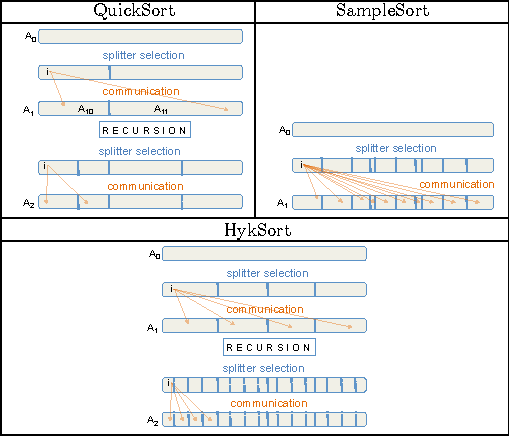
\includegraphics[width=0.7\linewidth]{images/ch_3/hyksort.pdf}}
    \caption{Communication pattern of Hyksort algorithm compared to a parallel Sample Sort, as well as a Quicksort over a hypercube, adapted from \cite{sundar2013hyksort}. We see that HykSort results in a lower communication overhead than Sample Sort.}
    \label{fig:chpt:3:sec:0:hyksort}
\end{figure}


Figure \ref{fig:chpt:3:sec:0:single_node_scaling} shows the scaling of our software, `Bempp-Tree', on a single node as time limitations inhibited multi-node experiments. In the left figure compare the performance of linear trees constructed using our software with the pointer-based trees constructed using the functionality of ExaFMM-t the leading single-node implementation of the kiFMM. We limit this comparison to uniform trees as they don't offer adaptive functionality. In the right figure we show weak scaling for fixed 1e6 points per MPI process for adaptive and uniform trees. We observe that there is a constant overhead in constructing adaptive trees, this comes from having to recursively refine blocks from the block tree by counting how many points they contain. The significant jump when using 8 MPI processes is likely due to the number of MPI processes exceeding the number of cores available on the Intel i7-9750 processor used for the experiments. Our performance in the single-node case is excellent, where we're able to generate an octree with 8e6 points, with a depth of 5, in approximately 13.5s. A marked improvement over ExaFMM-T, and demonstrative of the power of a bottom up approach in comparison to a pointer based approach used by that software. Multi-node experiments are required to assess the performance of our library in comparison to other state of the art tree libraries \cite{sampath2008dendro,BursteddeWilcoxGhattas11}. However, as our approach closely follows theirs we don't expect performance to be significantly different.

\begin{figure}[h]
  \centering
  \begin{minipage}[b]{0.45\textwidth}
    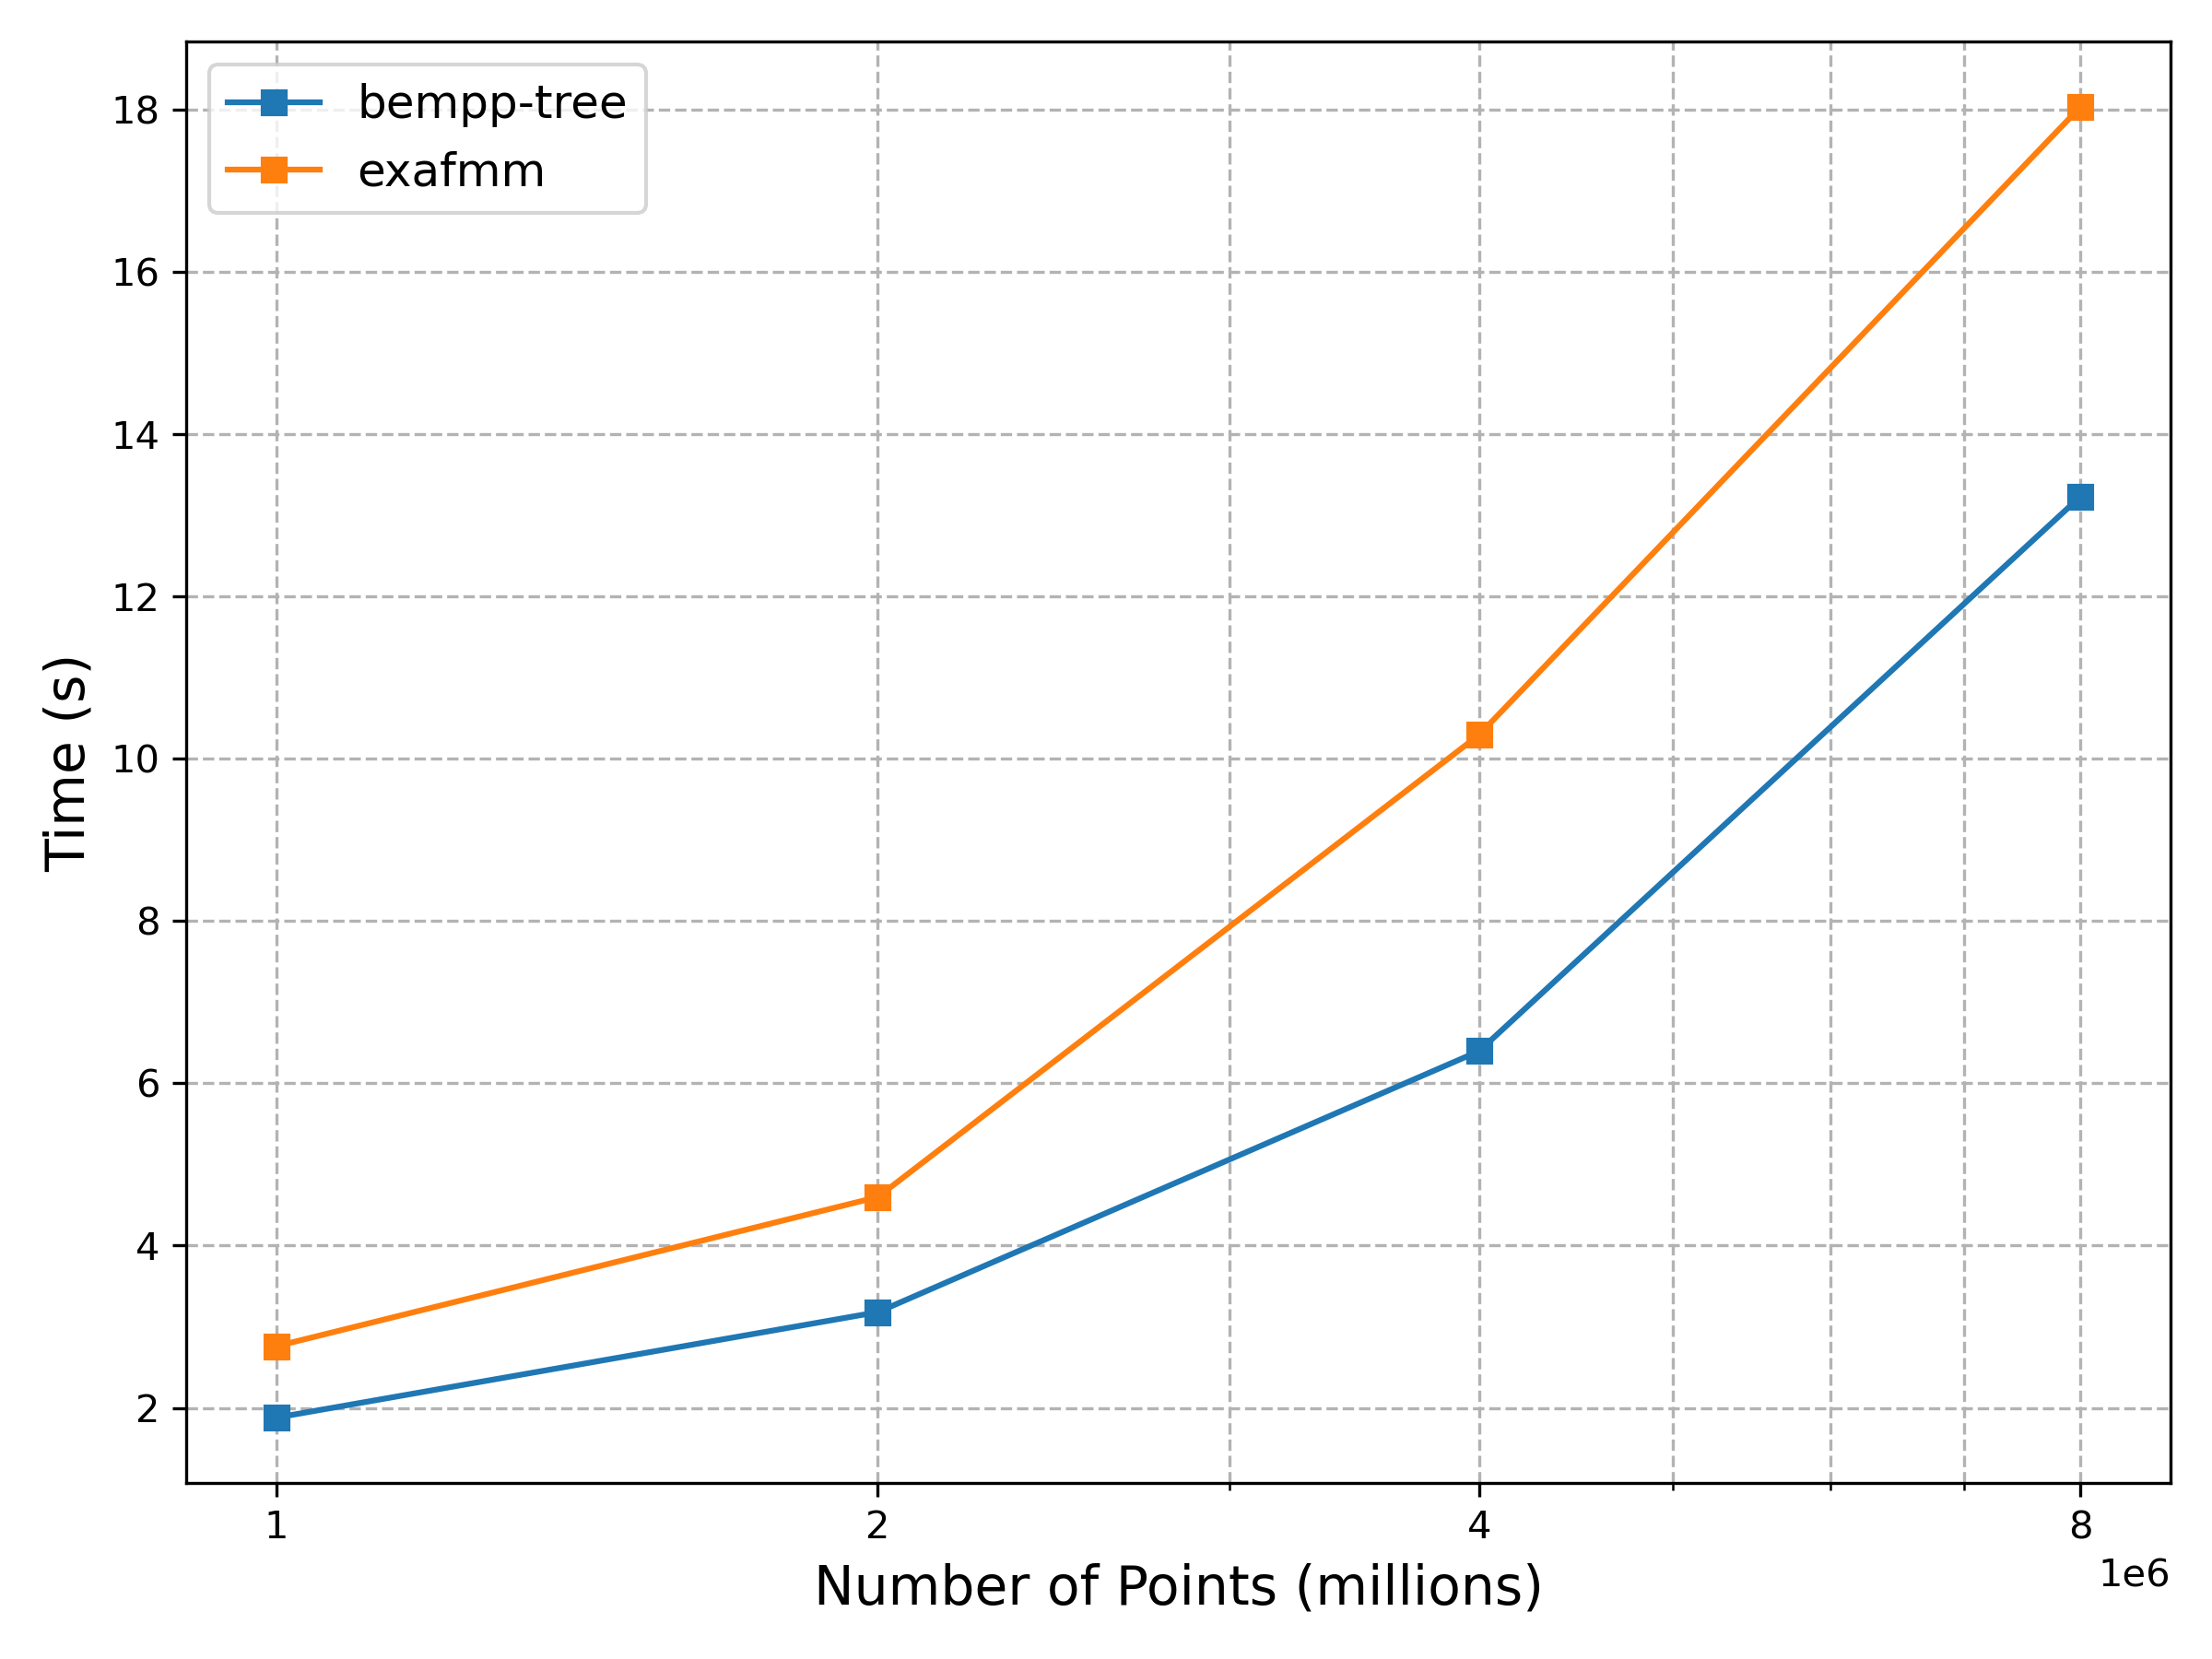
\includegraphics[width=\textwidth]{images/ch_3/single_node_scaling.png}
  \end{minipage}
  \hfill
  \begin{minipage}[b]{0.45\textwidth}
    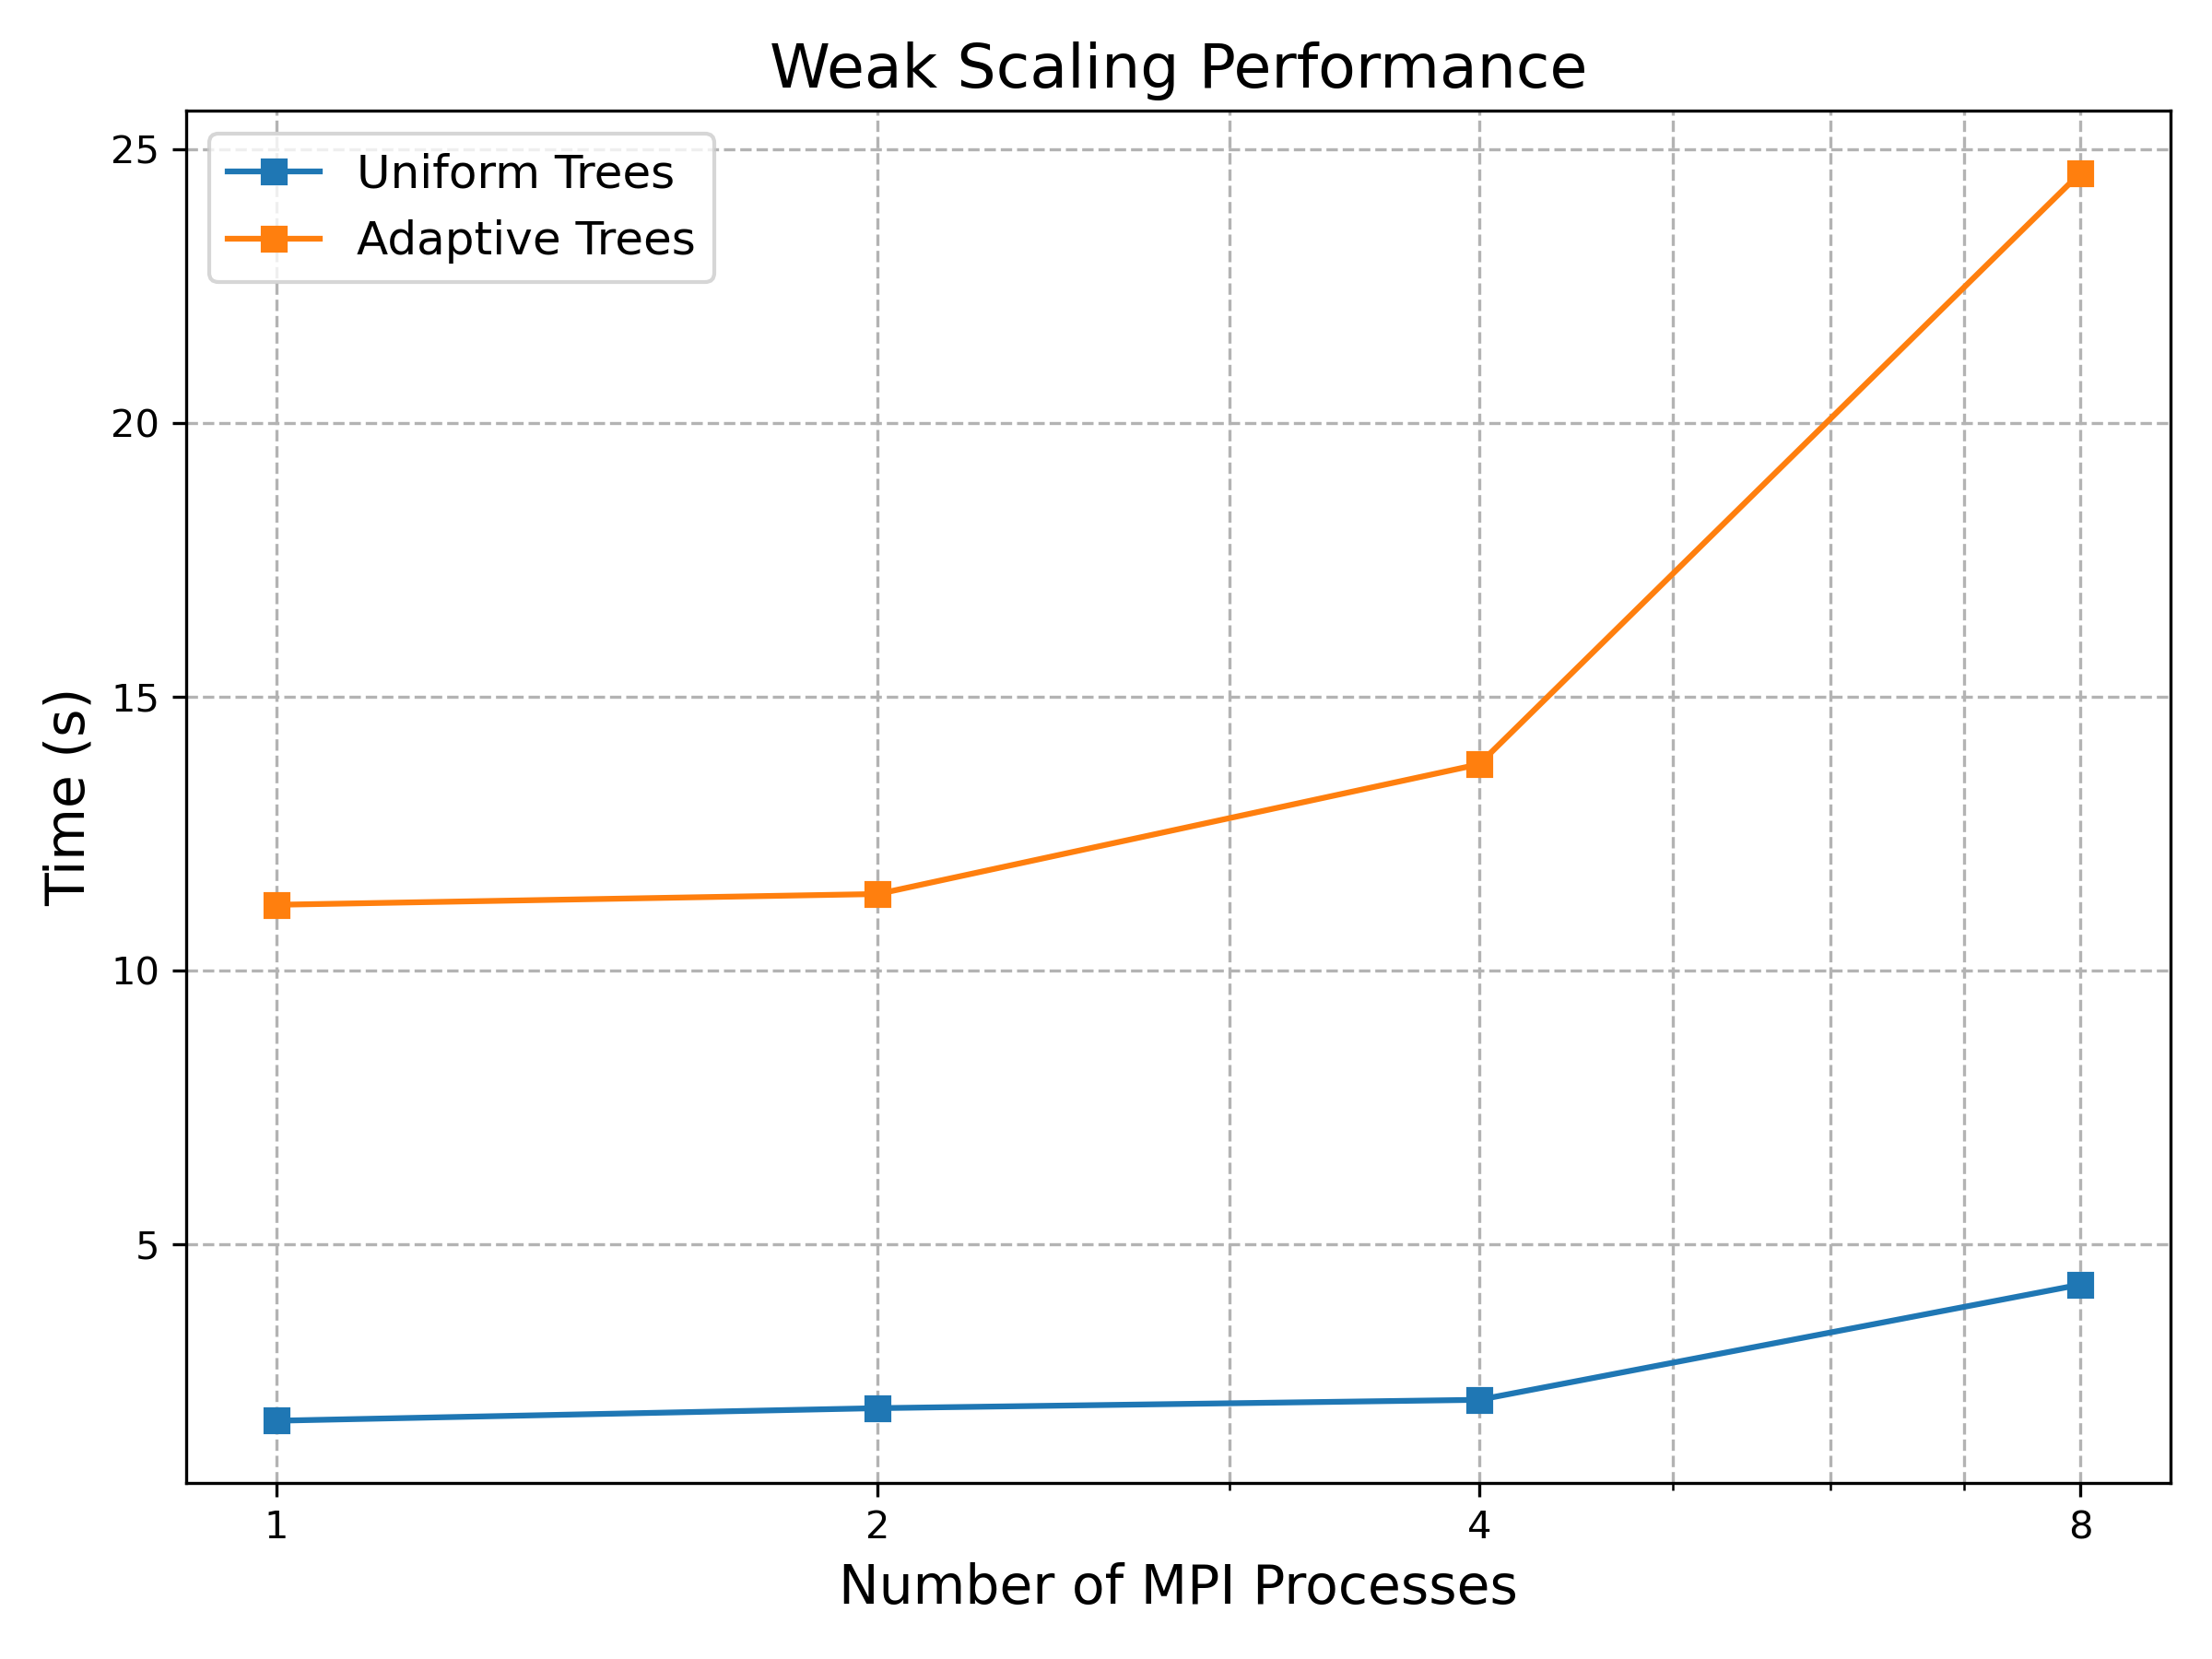
\includegraphics[width=\textwidth]{images/ch_3/weak_scaling_graph.png}
  \end{minipage}
\caption{The left figure shows the runtime of creating uniform trees on a single node in Bempp-Tree, in comparison to ExaFMM-T. The right figure shows weak scaling (over cores on a single node) of creating uniform and adaptive trees with Bempp-Tree, where each MPI process is given 1e6 points. The uniform trees are partitioned to a depth of 5, the adaptive trees have at most 150 particles in their leaf boxes. Experiments were taken on an Intel i7-9750H 6 core processor.}
\label{fig:chpt:3:sec:0:single_node_scaling}
\end{figure}

\subsection{Exposing Parallelism in A Distributed Memory FMM}

In the context of FMMs generating a distributed tree constitutes the first communication intensive phase. Further bottlenecks occur in the evaluation of the operators, most significantly in the evaluation of $T^{M2M}$ and $T^{M2L}$. To understand where these operators lead to communication bottlenecks, and how these can be overcome in practical implementations, we now introduce terminology relevant to distributing the FMM on parallel machines. We build upon the discussion first presented in Section 3 of \cite{Lashuk2012}, and use the same terminology.

Given a partition of a global tree $T$, as described above, such that each compute node $k$ contains a disjoint subset of leaves arranged in Morton order, $T_k$ we define a \textit{Locally Essential Tree} (LET) for compute node $k$ as the union of interaction lists for all its owned leaves, as well as their ancestors,

\begin{flalign}
    \text{LET}(k) := \cup_{N \in T_k \cup \text{Ancestors}(T_k)} \text{InteractionList}(N)
    \label{eq:chpt:3:sec:0:let}
\end{flalign}

We denote the region controlled by MPI process $k$ as $\Omega_k$, from the properties of Morton keys (see app. \ref{app:morton}) this is defined by the smallest and largest Morton key they hold. Using an MPI\_AllGather collective, we exchange information about the bounds of each MPI process globally. Following this, ancestors are added to each $T_k$ for the leaf nodes they control. In order to communicate `ghost octants', i.e. octants which are relied upon by the translation operators acting upon each $T_k$ but are not held locally, we introduce the concept of `Contributor' and `User' compute nodes,

\begin{enumerate}
    \item Contributor compute nodes for an octant $N \in T$ are
    \[
        \mathcal{P}_c(N) := k \in 1...p : N \text{ overlaps with } \Omega_k
    \]
    \item User compute nodes of an octant $N \in T$ are
    \[
        \mathcal{P}_u(N) := k \in 1...p : \text{ Parent($N$) or Neighbours ($N$) overlaps with } \Omega_k
    \]
\end{enumerate}

We denote the set of octants which compute node $k$ contributes and which process $k'$ uses as $I_{k k'}$. These are communicated and inserted into each compute node's local tree in order to complete the construction of its LET. Consider the potential generated by the sources enclosed by some octant $N$. In order to evaluate the potential outside the volume covered by $\text{Neighbours}(\text{Parent})(N)$ one doesn't need the multipole expansions, or sources, associated with $N$ as an ancestor of $N$ would be used instead. This ensures the correctness of this approach to constructing LETs.

Once an LET has been constructed, and particle information has been exchanged to user processors, the $T^{P2M}$ and $P2P$ operators don't require further communication. Lashuk et. al reason that this allows for the potential pipelining of $T^{P2M}$, $T^{M2M}$ and $T^{M2L}$, though they have not experimented with this. They identify the $T^{M2M}$ and $T^{M2L}$ operators as those requiring intensive communication phases during FMM evaluation. Beginning with $T^{M2M}$, the communication and calculation can be seen to progress in three steps,

\begin{enumerate}
    \item Firstly, source charges which are required for $P2P$ ar communicated with user MPI processes. As these will be relatively `local' communications within the context of a distributed memory machine, they use non-blocking point-to-point `Isend' functions for this step.
    \item Secondly, the multipole coefficients are summed for the octants on the coarser level.
    \item Thirdly, the multipole coefficients are communicated to user octants, as each MPI rank has only a partial sum for the octants at the parent level of each octant.
\end{enumerate}

During the downward pass Lashuk et. al.'s scheme doesn't require any further communication as each MPI process has all the multipole data, as well as point data, to compute the FMM for its locally held particles in parallel. The complexity of the communication of this scheme is given as $O(\sqrt{n_p}(N/n_p)^{2/3})$ where $n_p$ is the total number of MPI processes and $N$ is the number of particles for octrees created in $\mathbb{R}^3$. This complexity applies as upper bound for non-uniform point distributions.

Ibeid et. al \cite{Ibeid2016} propose an alternative communication scheme that achieves a tighter complexity bound of $O(\log(n_p) + (N/n_p)^{2/3})$. They rely on an alternative abstraction for handling the tree, by splitting it into a `global tree' and `local tree'. Their scheme is illustrated in Figure \ref{fig:chpt:3:sec:0:ibeid}, which describes a uniformly refined tree created for uniform point distributions\footnote{This is proved for uniform point distributions, and a uniformly refined octree in \cite{Ibeid2016}, but is also demonstrated to apply to non-uniform distributions.}, which we've adapted from Figure 3 in \cite{Ibeid2016}. Here a global tree is constructed such that the \textit{root node} of the tree on each MPI process is \textit{leaf node} of the global tree. The depth of the global tree, defined by $L_{\text{global}}$ in fig \ref{fig:chpt:3:sec:0:ibeid}, is thus defined by the number of MPI processes and is therefore $O(\log(n_p))$. The depth of the local tree is defined by the particles belonging to the MPI process and is seen to be $O(\log(N/n_p))$. By splitting the tree in this way, the communications during the $T^{M2M}$ and $T^{M2L}$ operators can be split into `global' and `local' phases. At the leaf nodes of the global tree, which starts at level $L_{\text{global}}$, after $T^{M2M}$ is performed, 8 neighbouring MPI processes contain the same information for boxes at $L_{\text{global}}-1$. Therefore, only one of them has to perform communications for the $T^{M2M}$ operation for the next level, proceeding recursively until the root of the global tree is reached. This corresponds to an 8-fold redundancy in the communication scheme proposed by Lashuk et. al. Using this, the number of communications at coarser global tree levels for each box stays constant at 7, and the communication complexity of the $T^{M2M}$ operator is proportional to the depth of the global tree $O(\log(n_p))$. The same redundancy can be used in reverse during the downward pass to communicate the multipole coefficients during $T^{M2L}$ on the global tree, which has the same complexity. We note however that in practice communications will occur between increasingly distant nodes at coarser levels of the tree, meaning that specific network topologies or interconnects would have an impact on practical performance.

Communications are still required during the downward pass of the local trees for computing $T^{M2L}$ and the $P2P$ operators. However, the communications are `local' in the sense that the same set of MPI processes will communicate with each other due to their overlapping LETs. This limits the number of processes to communicate with to $O(1)$ during these steps, as opposed to $O(n_p)$. However, as the number of boxes increases exponentially at finer tree levels, the amount of information being sent grows with increasing tree depth. This amounts to an increasing ratio of the surface to volume for finer boxes. The same is true for communicating the source point data for the $P2P$ operator. They find the number of boxes to be sent for $T^{M2L}$ at the $i^{th}$ level of the local tree to be $(2^i + 4)^3 - 8^i$ and $(2^i + 2)^3-8^i$ respectively. This can be seen by the fact that the interaction list for $T^{M2L}$ requires the communication of a halo that is 2 boxes wide, which adds 4 boxes per dimension, and similarly the $P2P$ requires the communication of a halo that is 1 box wide, which adds 2 boxes per dimension, and there are $8^i$ boxes at the $i^{th}$ level. Summing up the powers of four up to the depth of the local tree gives,

\begin{flalign}
    \sum_{i}^{\log_8(N/n_p)} 4^i = (N/n_p)^{\log(4)/\log(8)} = (N/n_p)^{2/3}
\end{flalign}

Giving a communication complexity of $O((N/n_p)^{2/3})$ for the local tree communications, and proving the bound provided by Ibeid et. al.

\begin{figure}[h]
    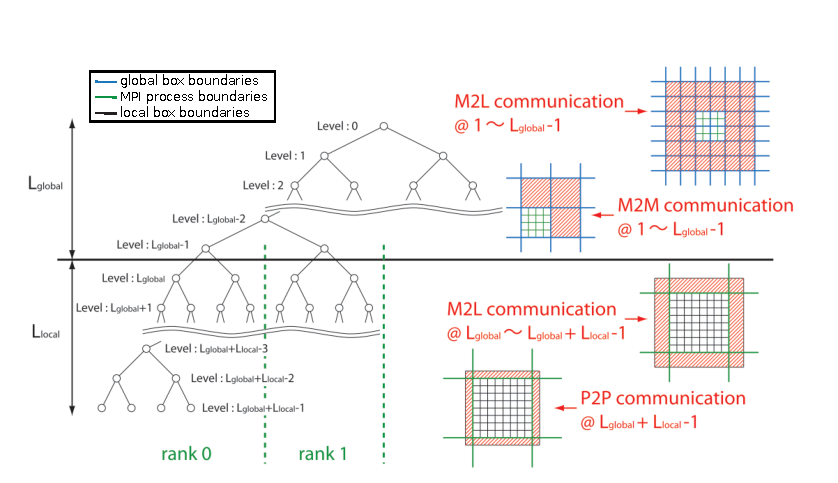
\includegraphics[width=\textwidth]{images/ch_3/ibeid.pdf}
    \caption{The tree structure shown here is a binary tree chosen for clarity by Ibeid et. al, this would be an octree in $\mathbb{R}^3$.}
    \label{fig:chpt:3:sec:0:ibeid}
\end{figure}

The near term priorities for our tree implementations are to implement the optimised communication scheme of Ibeid et. al., and compare its practical performance with the scheme provided by Lashuk et. al. Real architectures may offer discrepancies in performance from the that expected from complexity analysis as Ibeid et. al's approach results in communication between physically distant MPI processes and the scheme of Lashuk et. al. benefits from being simpler to implement, with low-effort opportunities for further optimisations through operation pipelining and has been demonstrated to scale well to thousands of MPI processes, with billions of points.
\label{chpt:3:sec:0:octrees}
\section{Fast Field Translations}
As noted in Chapter \ref{chpt:2:sec:2}, the $T^{M2L}$ is the most computationally intensive phase of an FMM implementation. In this section we describe two major approaches to accelerate its computation, chiefly a numerical compression scheme based on taking an SVD and relying on the low-rank nature of $T^{M2L}$, and secondly an `exact' method that relies on an FFT to redue the complexity of the convolution represented by $T^{M2L}$. We have implemented both via our software `Bempp-Field'\footnote{https://github.com/bempp/bempp-rs/tree/main/field}, and we use this section to describe the relative merits of these approaches, implementation challenges, as well as open questions which remain. We find that the FFT approach, which has been demonstrated to perform well in single node \cite{wang2021exafmm} as well as multi node \cite{malhotra2015pvfmm} to be our favoured approach. We propose new algorithm for its implementation, and offer some benchmarks for its performance in a single-node setting relative to the state of the art \cite{wang2021exafmm,malhotra2015pvfmm} which rely on a similar approach.



\subsection{SVD Field Translations}

In order to uniquely label M2L interactions we introduce transfer vectors $t = (t_1, t_2, t_3)$, $t \in \mathbb{Z}^3$. They describe the relative positioning of two boxes, $X$ and $Y$, in a hierarchical tree and computed from their centres $t = \frac{c_x - c_y}{w}$ where $w$ is the box width.

Consider the application of $T^{M2L}$, to a given multipole expansion $q$, where our goal is to compute the check potential $\phi$,

\begin{flalign}
    \phi = T^{M2L} q
\end{flalign}


As $T^{M2L}$ is known to be low-rank, it can be optimally approximated with an SVD,

\begin{flalign}
    \tilde{\phi} = U_k \Sigma_k V_k^T q
\end{flalign}

where $k$ indicates the rank of $T^{M2L}$, i.e. the smallest non-zero singular value. This can be shown to be an optimal approximation to $K$ \cite{Trefethen1997}. For homogenous, translationally invariant kernels we see from Table \ref{table:chpt:2:sec:1:m2l_optimisations} that there are at most 316 unique translation vectors corresponding to $T^{M2L}$ operations in $\mathbb{R}^3$. Stacking their corresponding discrete matrices column wise,

\begin{flalign}
    T^{M2L}_{\text{fat}} &= \left [ T^{M2L}_1, ..., T^{M2L}_{316} \right ] \\
    &= U \Sigma \left [ V^{T}_1, ..., V^{T}_{316} \right ]
    \label{eq:chpt:3:sec:1:subsec:1:m2l_fat}
\end{flalign}

or row-wise,

\begin{flalign}
    T^{M2L}_{\text{thin}} &= \left [ T^{M2L}_1; ...; T^{M2L}_{316} \right ] \\
    &= \left [ R^{T}_1; ...; R^{T}_{316} \right ]  \Lambda S^T
    \label{eq:chpt:3:sec:1:subsec:1:m2l_thin}
\end{flalign}


we note that,

\begin{flalign}
    T^{M2L}_{\text{thin}}  = (T^{M2L}_{\text{fat}})^T
\end{flalign}

for such kernels which are symmetric. Having computed these two SVDs we can reduce the application cost of a given $T^{M2L}_i$ between two boxes,

\begin{flalign}
    T^{M2L}_i q = R_i\Lambda S^T q
    \label{eq:chpt:3:sec:1:subsec:1:single_svd}
\end{flalign}

Using the fact that $S$ is unitary, i.e. $S^TS = I$, we can insert this into equation (\ref{eq:chpt:3:sec:1:subsec:1:single_svd}) to find,

\begin{flalign}
    T^{M2l}_{i} q &= R^{(i)}\Lambda S S^T S^T q \\
    &= T^{M2L}_{i} SS^T q \\
    &= U \Sigma V^{T}_i SS^T q \\
\end{flalign}


Now using that $U$ is also unitary such that $U^TU = I$, we find

\begin{flalign}
    T^{M2L}_i q &= UU^T U \Sigma V^{T}_i SS^T q \\
    &= U [U^T U \Sigma V^{T}_i S] S^T q \\
    &= U[U^T T^{M2L}_i S] S^T q
\end{flalign}


The bracketed terms can be calculated using the rank $k$ approximation from the SVD,

\begin{flalign}
    [U^T T^{M2L}_i S] &= \Sigma V^{T}_i S\\
    &= U^T R_{i} \Lambda
    \label{eq:chpt:3:sec:1:subsec:1:compressed_m2l}
\end{flalign}


We call equation (\ref{eq:chpt:3:sec:1:subsec:1:compressed_m2l}) the \textit{compressed $T^{M2L}$ operator}.

\begin{flalign}
    C^k_i = U^T T^{M2L}_i S
    \label{eq:chpt:3:sec:1:subsec:1:compressed_m2l_2}
\end{flalign}

This matrix can be precomputed for each unique interaction. Therefore in the kernels considered in this exposition, it must be computed at most 316 times, with corresponding pre-computations for kernels with different properties.

The application of $T^{M2L}$ can now be broken down into four steps.


\begin{enumerate}
    \item Find the `compressed multipole expansion'
    \[
    q_c = S^T q
    \]
    \item Compute the `compressed check potential', where the sum is taken over all boxes which have an applicable $T^{M2L}$ operator.
    \[
    \phi_c = \sum C^k_i q_c
    \]
    \item Post process to recover an uncompressed check potential
    \[
    \phi = U \phi_c
    \]
    \item Finally, calculate the local expansion from the check potential as done previously in Section \ref{chpt:2:sec:2}.
\end{enumerate}


The rank behaviour of $T^{M2L}$ has been assumed to be low-rank throughout this thesis, and therefore amenable to compression. However it remains an open question as to the exact rank behaviour of a given kernel in practice. This has consequences for real implementations, as if we are able to effectively cut-off the rank $k$ with $\kappa \ll k$ we may be able to reduce the complexity of the SVD based scheme $T^{M2L}$ further. Figure [RANK FIGURE] shows the effective rank behaviour of the Laplace kernel for different expansion orders ...

- Analytical considerations to investigate the rank behaviour of the kernel could be used to identify the cut-off ranks $\kappa$ based on the transfer vector.

- Rank experiment for Laplace, different orders, where is the cut-off, and what is the accuracy?

Furthermore, practical implementations can re-formulate the SVD based scheme to increase the computational intensity\footnote{The computational intensity is short hand for the ratio of computations to memory accesses, i.e. flops/bytes.} of the operation. As presented above, each box $B$ will have to compute $T^{M2L}$ for each box in its relevant halo, up to 189 times in $\mathbb{R}^3$. For each of these applications, $B$ will have to look up the appropriate compressed $T^{M2L}$ from memory in this naive scheme. Matrix vector products are handled by BLAS level 2 operations, however by taking advantage of BLAS level 3 operations we can increase the ratio of compute/memory access. We do so in our implementation by blocking together \textit{all} the right hand sides, i.e. multipole expansions, which share a given translation vector $t$ and compute their compressed check potentials in a single matrix-matrix product. This has a dramatic effect on the runtime of our software as shown in Figure [NAIVE VS BLOCKED FIGURE].

We note that the precomputation for this approach relies on an SVD of two relatively large matrices in (\ref{eq:chpt:3:sec:1:subsec:1:m2l_fat}) and (\ref{eq:chpt:3:sec:1:subsec:1:m2l_thin}) where we use the `greedy' DGESVD provided by LAPACK. For the Laplace kernel, which is translationally invariant and homogenous, precomputation times are shown in Figure [PRECOMPUTE TIME FIGURE]. However, for kernels which are translationally invariant but not homogenous, these must be computed for each level of the octree which can have a significant impact on setup time for the FMM, dominating the tree setup time as well as the algorithm runtime. This could be alleviated with alternative implementations that make use of randomised algorithms, which have been shown to have considerably faster runtimes for a given compression rank \cite{halko2011finding}, though we haven't explored this as of date.


\subsection{FFT Field Translations}

From the structure of our kernels of interest (\ref{eq:chpt:2:sec:0:laplace_kernel}), as well as the fact that our equivalent densities and check potentials are arranged on a regular grid (fig. \ref{fig:chpt:2:sec:1:translations}), we notice that the calculation of the downward check potential during $T^{M2L}$ is a convolution,


\begin{flalign}
    \phi = (K \ast q)(x) = \int_{y^{B, d}} K(x-y)q^{A, u}(y)dy
    \label{eq:chpt:3:sec:1:subsec:2:m2l_convolution}
\end{flalign}

When translating the multipole expansion at a box $A$ to a box $B$. From Fourier theory, the property of the Fourier transforms of a convolution is that they are the product of two individual transforms,

\begin{flalign}
    \mathcal{F} \{K \ast q\}(k) = \mathcal{F}\{K\}(k) \cdot \mathcal{F}\{q\}(k)
\end{flalign}

where $k$ denotes the frequencies in Fourier space. We therefore find that the check potential can be computed as,

\begin{flalign}
    \phi(x) = \mathcal{F}^{-1}\{ \mathcal{F}\{K\}(k) \cdot \mathcal{F}\{q\}(k)  \} (x)
\end{flalign}

In practice for the kiFMM the sequence corresponding to $K$ must contain all the unique evaluations of the kernel (\ref{eq:chpt:2:sec:0:laplace_kernel}) between a source box $A$ and a target box $B$. This sequence is constructed with the help of an ancillary data structure known as a `convolution grid'.

We illustrate the construction of the sequences that are required for an FFT based $T^{M2L}$ in $\mathbb{R}^2$, however they are directly applicable to $\mathbb{R}^3$. Consider Figure \ref{fig:chpt:3:sec:1:subsec:2:translations}, which shows a source and target box, each of which is annotated with source equivalent points $y_i$ and target check points, $x_i$, for a $P=2$ expansion.

\begin{figure}
    \centering
    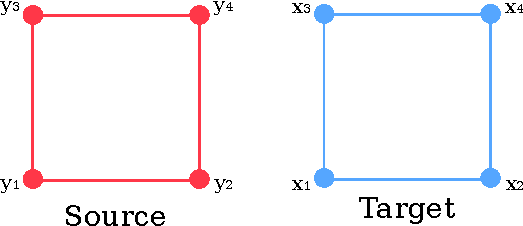
\includegraphics[width=0.6\textwidth]{images/ch_3/m2l_source_target.pdf}
    \caption{A source and target box, with source and target locations on the repsective equivalent and check surface annotated..}
    \label{fig:chpt:3:sec:1:subsec:2:translations}
\end{figure}

The equivalent surface around the source box is \textit{embedded} within a convolution grid, as shown in Figure \ref{fig:chpt:3:sec:1:subsec:2:embed_surface_grid}, such that the number of points on a convolution grid is $P^3$ in $\mathbb{R}^3$ and $P^2$ in $\mathbb{R}^2$ respectively.

\begin{figure}
    \centering
    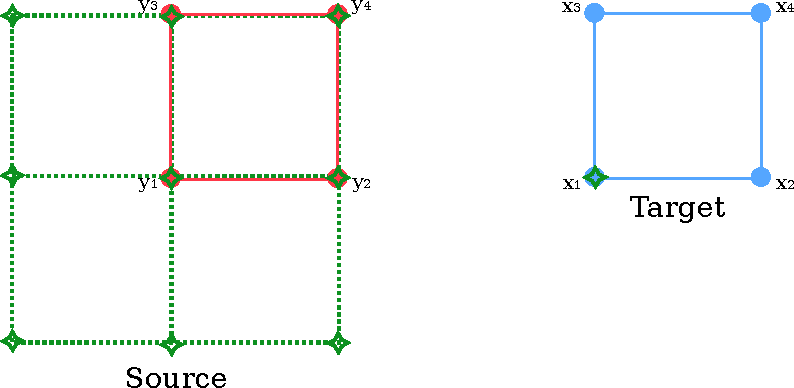
\includegraphics[width=0.6\textwidth]{images/ch_3/embed_surface_grid.pdf}
    \caption{The source equivalent surface is embedded within a (green) convolution grid. The points on the convolution grid are marked with diamonds. An additional diamond is placed on the target check surface, which identifies the point with which kernels are evaluated with respect to.}
    \label{fig:chpt:3:sec:1:subsec:2:embed_surface_grid}
\end{figure}

The unique kernel interactions between the source equivalent surface and the target check surface in (\ref{eq:chpt:3:sec:1:subsec:2:m2l_convolution}) are computed with respect to a single point on the target check surface and the points on the convolution grid. We then see that we must compute the convolution of two sequences in $\mathbb{R}^2$, illustrated in Figure \ref{fig:chpt:3:sec:1:subsec:2:convolution}. Here the first sequence is the unique kernel evaluations taken with respect to a fixed point on the target check surface, and the second sequence is the multipole expansion coefficients mapped to the convolution grid from the source box's equivalent surface. We proceed to take Fourier transforms via the FFT for both of these sequences, and compute their convolution via a Hadamard product.

\begin{figure}
    \centering
    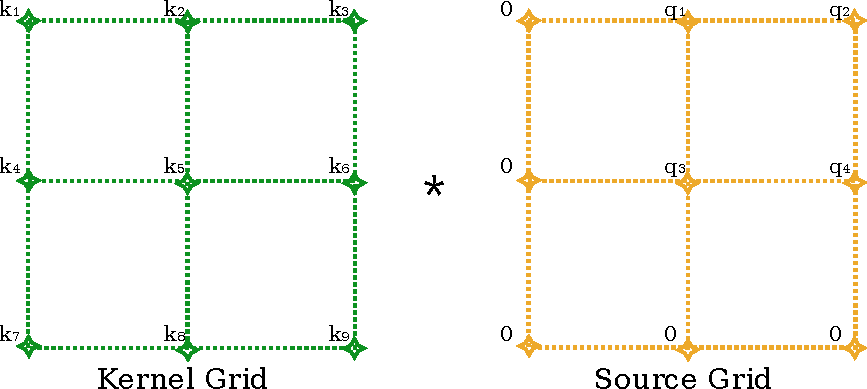
\includegraphics[width=0.6\textwidth]{images/ch_3/convolution.pdf}
    \caption{A Hadamard product is computed between the Fourier transforms sequence of unique kernel evaluations and the multipole expansion coefficients which are also placed on the convolution grid.}
    \label{fig:chpt:3:sec:1:subsec:2:convolution}
\end{figure}

Computing this Hadamard product results in another sequence illustrated in Figure \ref{fig:chpt:3:sec:1:subsec:2:check_potential}, where we have taken care to `flip' the sequence corresponding the unique kernel evaluations as required by the definition of a convolution. We find the final check potentials by taking the inverse Fourier transform of it.

\begin{figure}
    \centering
    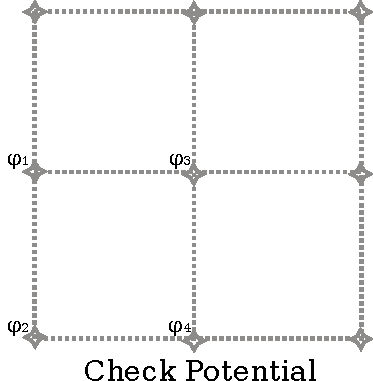
\includegraphics[width=0.3\textwidth]{images/ch_3/check_potential.pdf}
    \caption{The result of the convolution illustrated in Figure \ref{fig:chpt:3:sec:1:subsec:2:convolution}, on the convolution grid. We only identify locations that correspond to check potentials, as the other entries will contain results which are not required, corresponding to redundant computations with this method.}
    \label{fig:chpt:3:sec:1:subsec:2:check_potential}
\end{figure}

We note that although we rely on the existence of a convolution grid to compute the required sequences, in practice we do not compute or store it. We simply require a mapping between the index locations of points on the equivalent surfaces to their corresponding positions on a convolution grid.

Expressed alternatively, we can represent the points on an equivalent surface, $y \in y^{B, u}$, by their respective indices $y_{i, j, k}$ when in $\mathbb{R}^3$. The elements corresponding to the unique kernel interactions are then,

\begin{flalign}
    K_{ijk} = K(x_{000} - y_{ijk})
\end{flalign}

where $x_{000}$ is the index of a point on the target equivalent surface with which the sequence is calculated with respect to. We choose the bottom left corner on the target surface, though in principle any point could be used, it would just amount to a translation of the convolution grid. This results in a 3D sequence $K[ ]$, with elements,

\begin{flalign}
    K[i, j, k] = K_{i, j, k}
\end{flalign}

Again the symmetries of kernels make the Fourier transforms of this quantity something that has the potential to be pre-computed and cached, in a similar way to which the SVD based $T^{M2L}$ could be cached. At runtime, we simply need to look up the corresponding sequence $\hat{K}_t[ ]$ corresponding to a transfer vector $t$ between a given source and target box, and compute the convolution as outlined above. The reduced complexity of the FFT in comparison to an SVD results in greatly faster pre-computation times (see fig. \ref{fig:chpt:3:sec:1:subsec:2:fft_m2l_precomputation} as opposed to fig. \ref{fig:chpt:3:sec:1:subsec:1:svd_m2l_precomputation}).

The Hadamard product has a low computational intensity\footnote{Ratio of flops to memory accesses.}, and naive implementations can be slow in practice regardless of the superior complexity of the FFT based $T^{M2L}$ in comparison to the compressed matrix vector products of the SVD approach outlined in the previous section especially when combined with optimisations to use BLAS3 operations. The authors of the leading multi-node bbFMM \cite{malhotra2015pvfmm} use a strategy of considering sets of siblings together, alongside explicit SIMD to increase the computational intensity of this operation. This approach is re-implemented by the authors of the leading single-node kiFMM \cite{wang2021exafmm}, though involves computes redundant $T^{M2L}$ translations. We explain briefly how this works below, before introducing our own approach which though similar, avoids these redundancies.

Consider a source box alongside its siblings in $\mathbb{R}^3$,

\begin{flalign}
    S = \cup_{i=1}^{N=8} S_i
\end{flalign}

For each unique $T^{M2L}$ we have a sequence $K[ ]$, and can pre-compute a sequence $\hat{K}[ ]$ corresponding to their Fourier transforms. Considering the sibling set $S$'s parent box, we can compute $T^{M2L}$ with respect to the neighbours of $S$'s parent. This results in $64 = 8 \times 8$ for translations between $S$ and the children in a particular neighbour of their parent, with corresponding sequences $\hat{K}[ ]$. We note that note all of these translations are necessarily required, the authors of \cite{malhotra2015pvfmm,wang2021exafmm} simply take the convolutions with respect to zero data used for the corresponding multipole expansion. When repeated for all of the neighbour's of $S$'s parent, we're left with a total of $1664 = 8 \times 8 \times 26$ applications of $T^{M2L}$ for a given sibling set $S$. Despite containing redundant calculations, the implementation is highly cache-optimised. The authors of \cite{malhotra2015pvfmm} proceed by iterating over each of $S$'s parent's neighbours - pulling out the $i^{th}$ frequency component from each - leading to a sequence of length $8 \times 8 \times 26$, they proceed by pulling out the $i^{th}$ frequency component of the Fourier transform of each sibling - leading to a sequence of length 8. The Hadamard product is found by computing 26 individual $8 \times 8$ operation using explicit SIMD. By iterating over $S$'s parent's neighbours in the outer loop the sequence of length $8 \times 8 \times 26$ can be held in memory for each subsequent sibling set.

This strategy is known to perform well. An experiment with the Laplace kernel, order $P=9$ expansions, and 1e6 source/target points takes at most 2.7s to evaluate $T^{M2L}$ on a 6 core Intel i7-9750H processor\footnote{Experiments were repeated 5 times, we report the maximum runtime.}. However, we note that the redundant computations can be reduced.

We begin by noting that for our kernels of interest correspond lead to 316 unique translation vectors $t$ with corresponding $T^{M2L}$ operators, however the majority of these operators correspond to reflections of each other. First introduced by Messner et. al \cite{messner2012optimized} in the context of an SVD based acceleration of $T^{M2L}$, where they attempt to reduce the size of the SVD required for the pre-computation in this approach, one can reduce the number of transfer vectors corresponding to \textit{unique} $T^{M2L}$ to just 16. In the original paper they aimed to demonstrate that with just 16 unique $T^{M2L}$ BLAS3 matrix-matrix products would further reduce the application time of the compressed $T^{M2L}$ operator, however as we demonstrate in Figure \ref{fig:chpt:3:sec:1:subsec:2:blas3}, we don't observe this to have a significant effect on the runtime of the matrix-matrix products of the sizes expected in a typical FMM, at least on modern processors as used during testing.

\begin{figure}
    \centering
    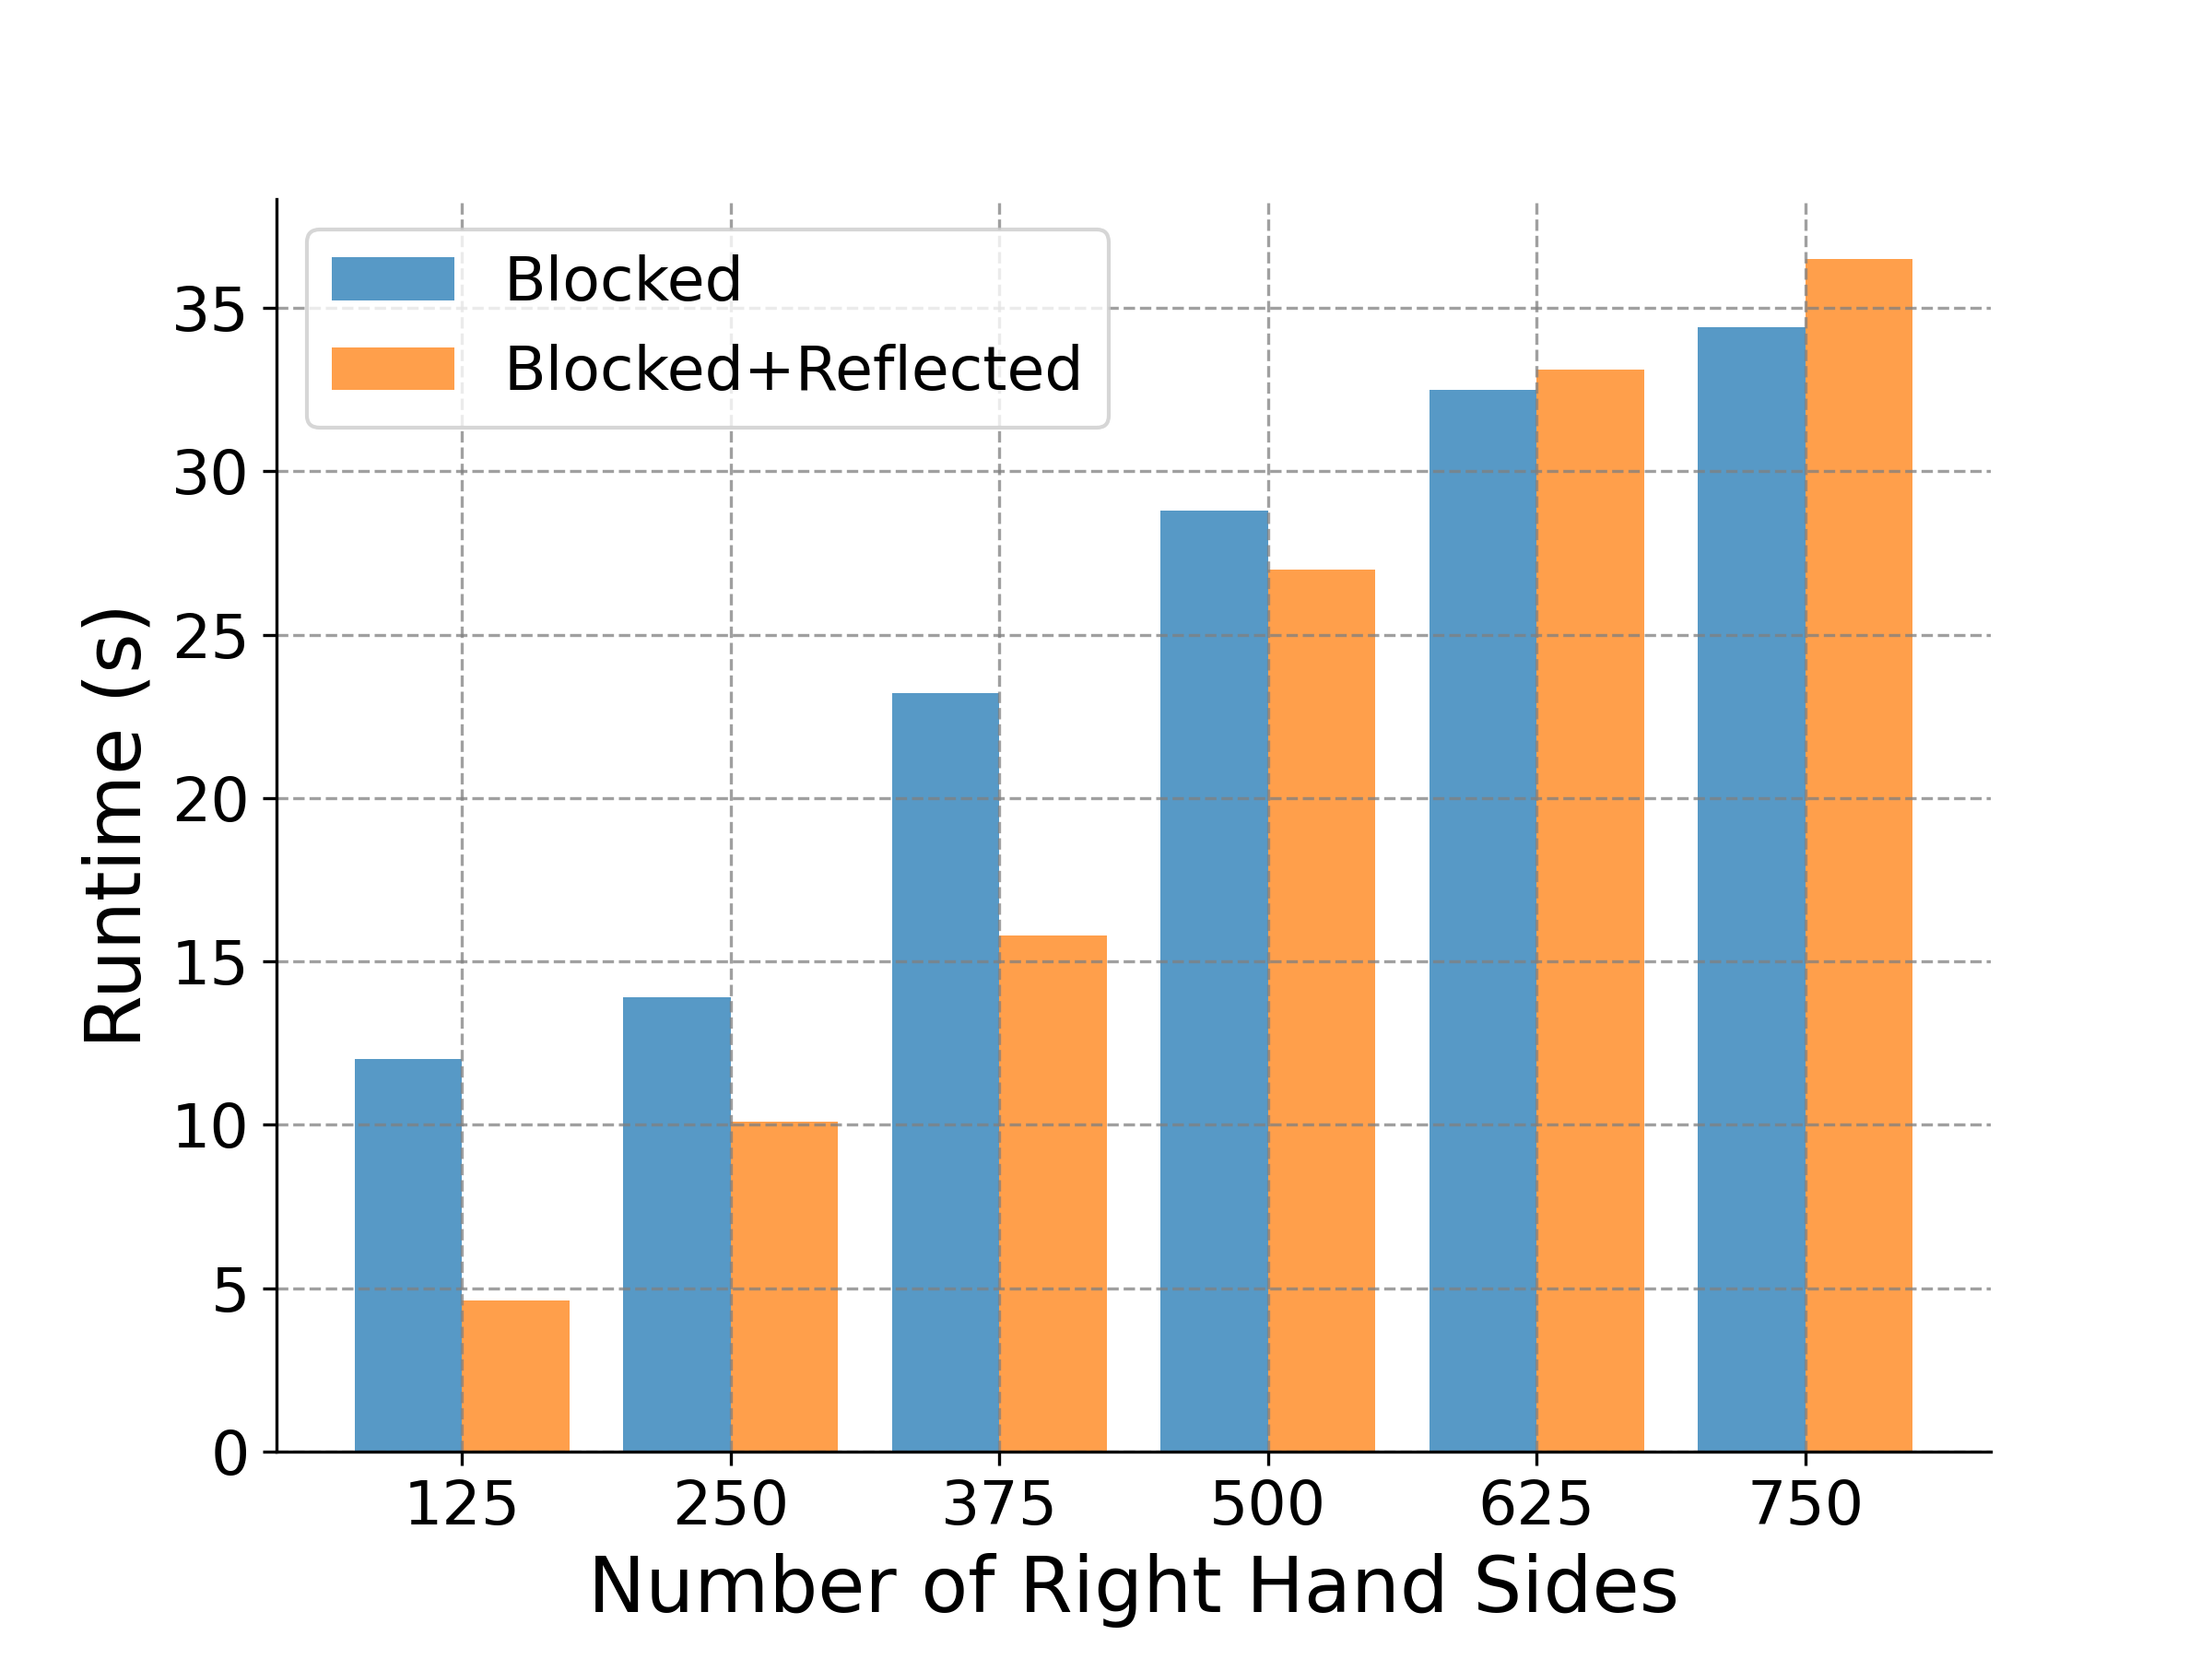
\includegraphics[width=0.6\textwidth]{images/ch_3/blas3.png}
    \caption{In this experiment we compared the runtime for blocking together matrix-matrix products corresponding to $T^{M2L}$ for each of 316 transfer vectors (labelled `Blocked'), to blocking together matrix-matrix products for each of a reduced set of just 16 unique transfer vectors (labelled `Blocked + Reflected'). The left matrix is a random dense matrix generated using double precision floating point numbers, with dimensions matching $T^{M2L}$ for expansion orders of 9, the right matrix is again a random dense matrix generated using double precision floating point numbers chosen to represent the multipole coefficients being translated. To estimate the runtime of application of the blocking approaches, we simply compute the matrix-matrix product with 20 times as many right hand sides ($316/16 = 19.75 \approx 20$) for the reduced blocking scheme, as the blocking scheme doesn't reduce the number of flops in this approach. The matrix-matrix product for the naively blocked scheme is correspondingly computed repeatedly in a loop of length 20, ensuring that both approaches have a matching number of flops. We find that for smaller numbers of right-hand sides, the reducing the set of transfer vectors to make more efficient use of BLAS3 matrix-matrix products does help significantly, however for larger numbers of right-hand sides greater than approximately 500, which is typical for the FMM, there is little difference with this optimisation. Experiments are taken on a 6 core Intel i7-9750 processor using Open BLAS, we report maximum runtimes over 5 runs for each set of parameters.}
    \label{fig:chpt:3:sec:1:subsec:2:blas3}
\end{figure}

In order to see how we arrive at 16 unique $T^{M2L}$ operators we introduce two symmetries, building upon the discussion in \cite{messner2012optimized}. They describe two planes of symmetry, axial and diagonal, when considering a source box $A$ and a target box $B$ during a given interaction specified by a $T^{M2L}$ operator. This is sketched for $\mathbb{R}^2$ for clarity in Figure \ref{fig:chpt:3:sec:1:subsec:2:symmetries}, where we show three sources $A$ with their respective transfer vectors, $t$, with respect to $B$. These boxes describe the equivalent/check surfaces described above for the kiFMM and the quadrature points are labelled by an index coordinate for an expansion of $P=2$. The axial planes of symmetry are given by $t_1 = 0$, $t_2 = 0$ and $t_3 = 0$ in $\mathbb{R}^3$, each dividing $\mathbb{R}^3$ into two parts centered on the target box $B$. Combining all three plane divides $\mathbb{R}^3$ into octants centered on $B$, we refer to $\mathbb{R}^3_+$ as the \textit{reference octant}. The diagonal planes of symmetry are given by $t_1 = t_2$, $t_1 = t_3$ and $t_2 = t_3$ in $\mathbb{R}^3$. We restrict ourselves to diagonal symmetries that lie in the reference octant. Combining the axial and diagonal symmetries we obtain a \textit{reference cone},

\begin{flalign}
    \mathbb{R}^3_{\text{sym}} = \{ \mathbb{R}^3_{\text{sym}} \subset \mathbb{R}^3 : t_1 \geq t_2 \geq t_3 \text{ with } t \in \mathbb{R}^3 \}
    \label{eq:chpt:3:sec:1:subsec:2:reference_cone}
\end{flalign}

We identify a subset of transfer vectors $T_{\text{sym}} = T \cap  \mathbb{R}^3_{\text{sym}}$ from which all transfer vectors for $B$ can be expressed as reflections around the axes of symmetry. Explicitly to find $t$ within $T_{\text{sym}}$, we apply the following rule

\begin{enumerate}
    \item A \textit{axial symmetry} given by say $t_1 = 0$ as shown in Figure \ref{fig:chpt:3:sec:1:subsec:2:symmetries}, we invert the corresponding component of the index coordinate
    \[
        \alpha \leftarrow (P-(\alpha_1-1), \alpha_2, \alpha_3) \text{ and } \beta \leftarrow (P-(\beta_1-1), \beta_2, \beta_3)
    \]
    \item A \textit{diagonal symmetry} given by say $t_1 = t_2$, w swap the corresponding components of the index coordinate as,
    \[
        \alpha \leftarrow (\alpha_2, \alpha_1, \alpha_3) \text{ and } \beta \leftarrow (\beta_2, \beta_1, \beta_3)
    \]
\end{enumerate}


Where as before $P$ stands for expansion order. When these rules are applied to the 316 unique transfer vectors for our kernels of interest, we find that $|T_{\text{sym}}|  = 16$.

\begin{figure}
    \centering
    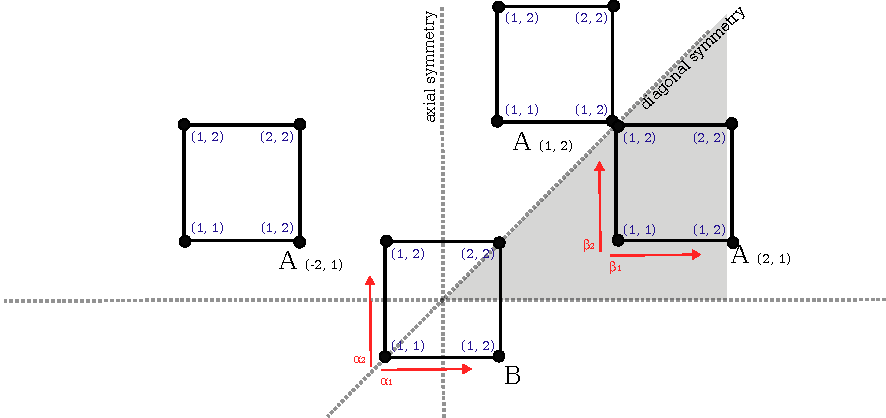
\includegraphics[width=\textwidth]{images/ch_3/symmetries.pdf}
    \caption{Here we show the axial and diagonal symmetries of three source boxes labelled $A$ with respect to a target box $B$ in $\mathbb{R}^2$ for expansion order $P=2$. The quadrature points are labelled with index coordinates taken with respect to the lower left corner of the box. The only transfer vector here the constraints of being in the `reference cone', which is shaded in grey, is $t=(2, 1)$ and therefore corresponds to the only $T^{M2L}$ that needs to be pre-computed. This figure is adapted from \cite{messner2012optimized} for the kiFMM as opposed to the bbFMM as originally presented.}
    \label{fig:chpt:3:sec:1:subsec:2:symmetries}
\end{figure}

Utilising this redundancy for the FFT accelerated $T^{M2L}$ means that one only has to precompute Fourier transform of Kernel sequences $K[]$ corresponding to transfer vectors in $T_{\textit{sym}}$. In order to reduce the number of flops required for computing $T^{M2L}$ during the algorithm we notice that $T^{M2L}$ is calculated for a box $B$ from a halo consisting of its interaction list, i.e. the children of $B$'s parent which it does not lie adjacent to. There is a conjugacy in this relationship meaning that if $A$ is in that set of boxes for $B$, then $B$ is correspondingly in that set of boxes for $A$. This means that we can `invert' the application of the $T^{M2L}$ operator. Instead of attempting to compute the check potential at $B$ from boxes $A$ in its halo, we can instead compute the convolutions corresponding to just 16 unique $T^{M2L}$ for the multipole coefficients at $B$ and scatter the resulting check potential to their corresponding boxes in $B$'s halo. This means that we are only computing 16 convolution operations with respect to each box, in comparison the 1664 as in previous implementations.

This transforms the problem into one that is bound by memory accesses. To alleviate this we take a similar approach to the state of the art softwares mentioned above, and consider sibling sets $S$ at a time. We iterate over sibling sets in parallel, pulling in references to $S$'s parent's neighbours' children into memory in each parallel thread. These constitute all the scatter locations for the check potentials computed for each box in $S$. By doing this however we reduce the number of cache-misses during the scatter operation as we an save all the corresponding check potentials to a box in $S$'s halo at once. For the same benchmark problem above we reported for the state of the art approach of \cite{malhotra2015pvfmm}, we compute $T^{M2L}$ in 6.8s \footnote{Experiments were repeated 5 times, we report the maximum runtime.}.

The effect of memory ordering and access on runtimes is clear, and significant, for this operation. As of writing are still working on an optimal memory ordering in the implementation of this approach, which if we are able to find would constitute a new algorithm for sparsifying $T^{M2L}$ via the FFT for algebraic FMMs discretised on regular grids, as the number flops in our approach is greatly reduced.

\begin{figure}
    \centering
    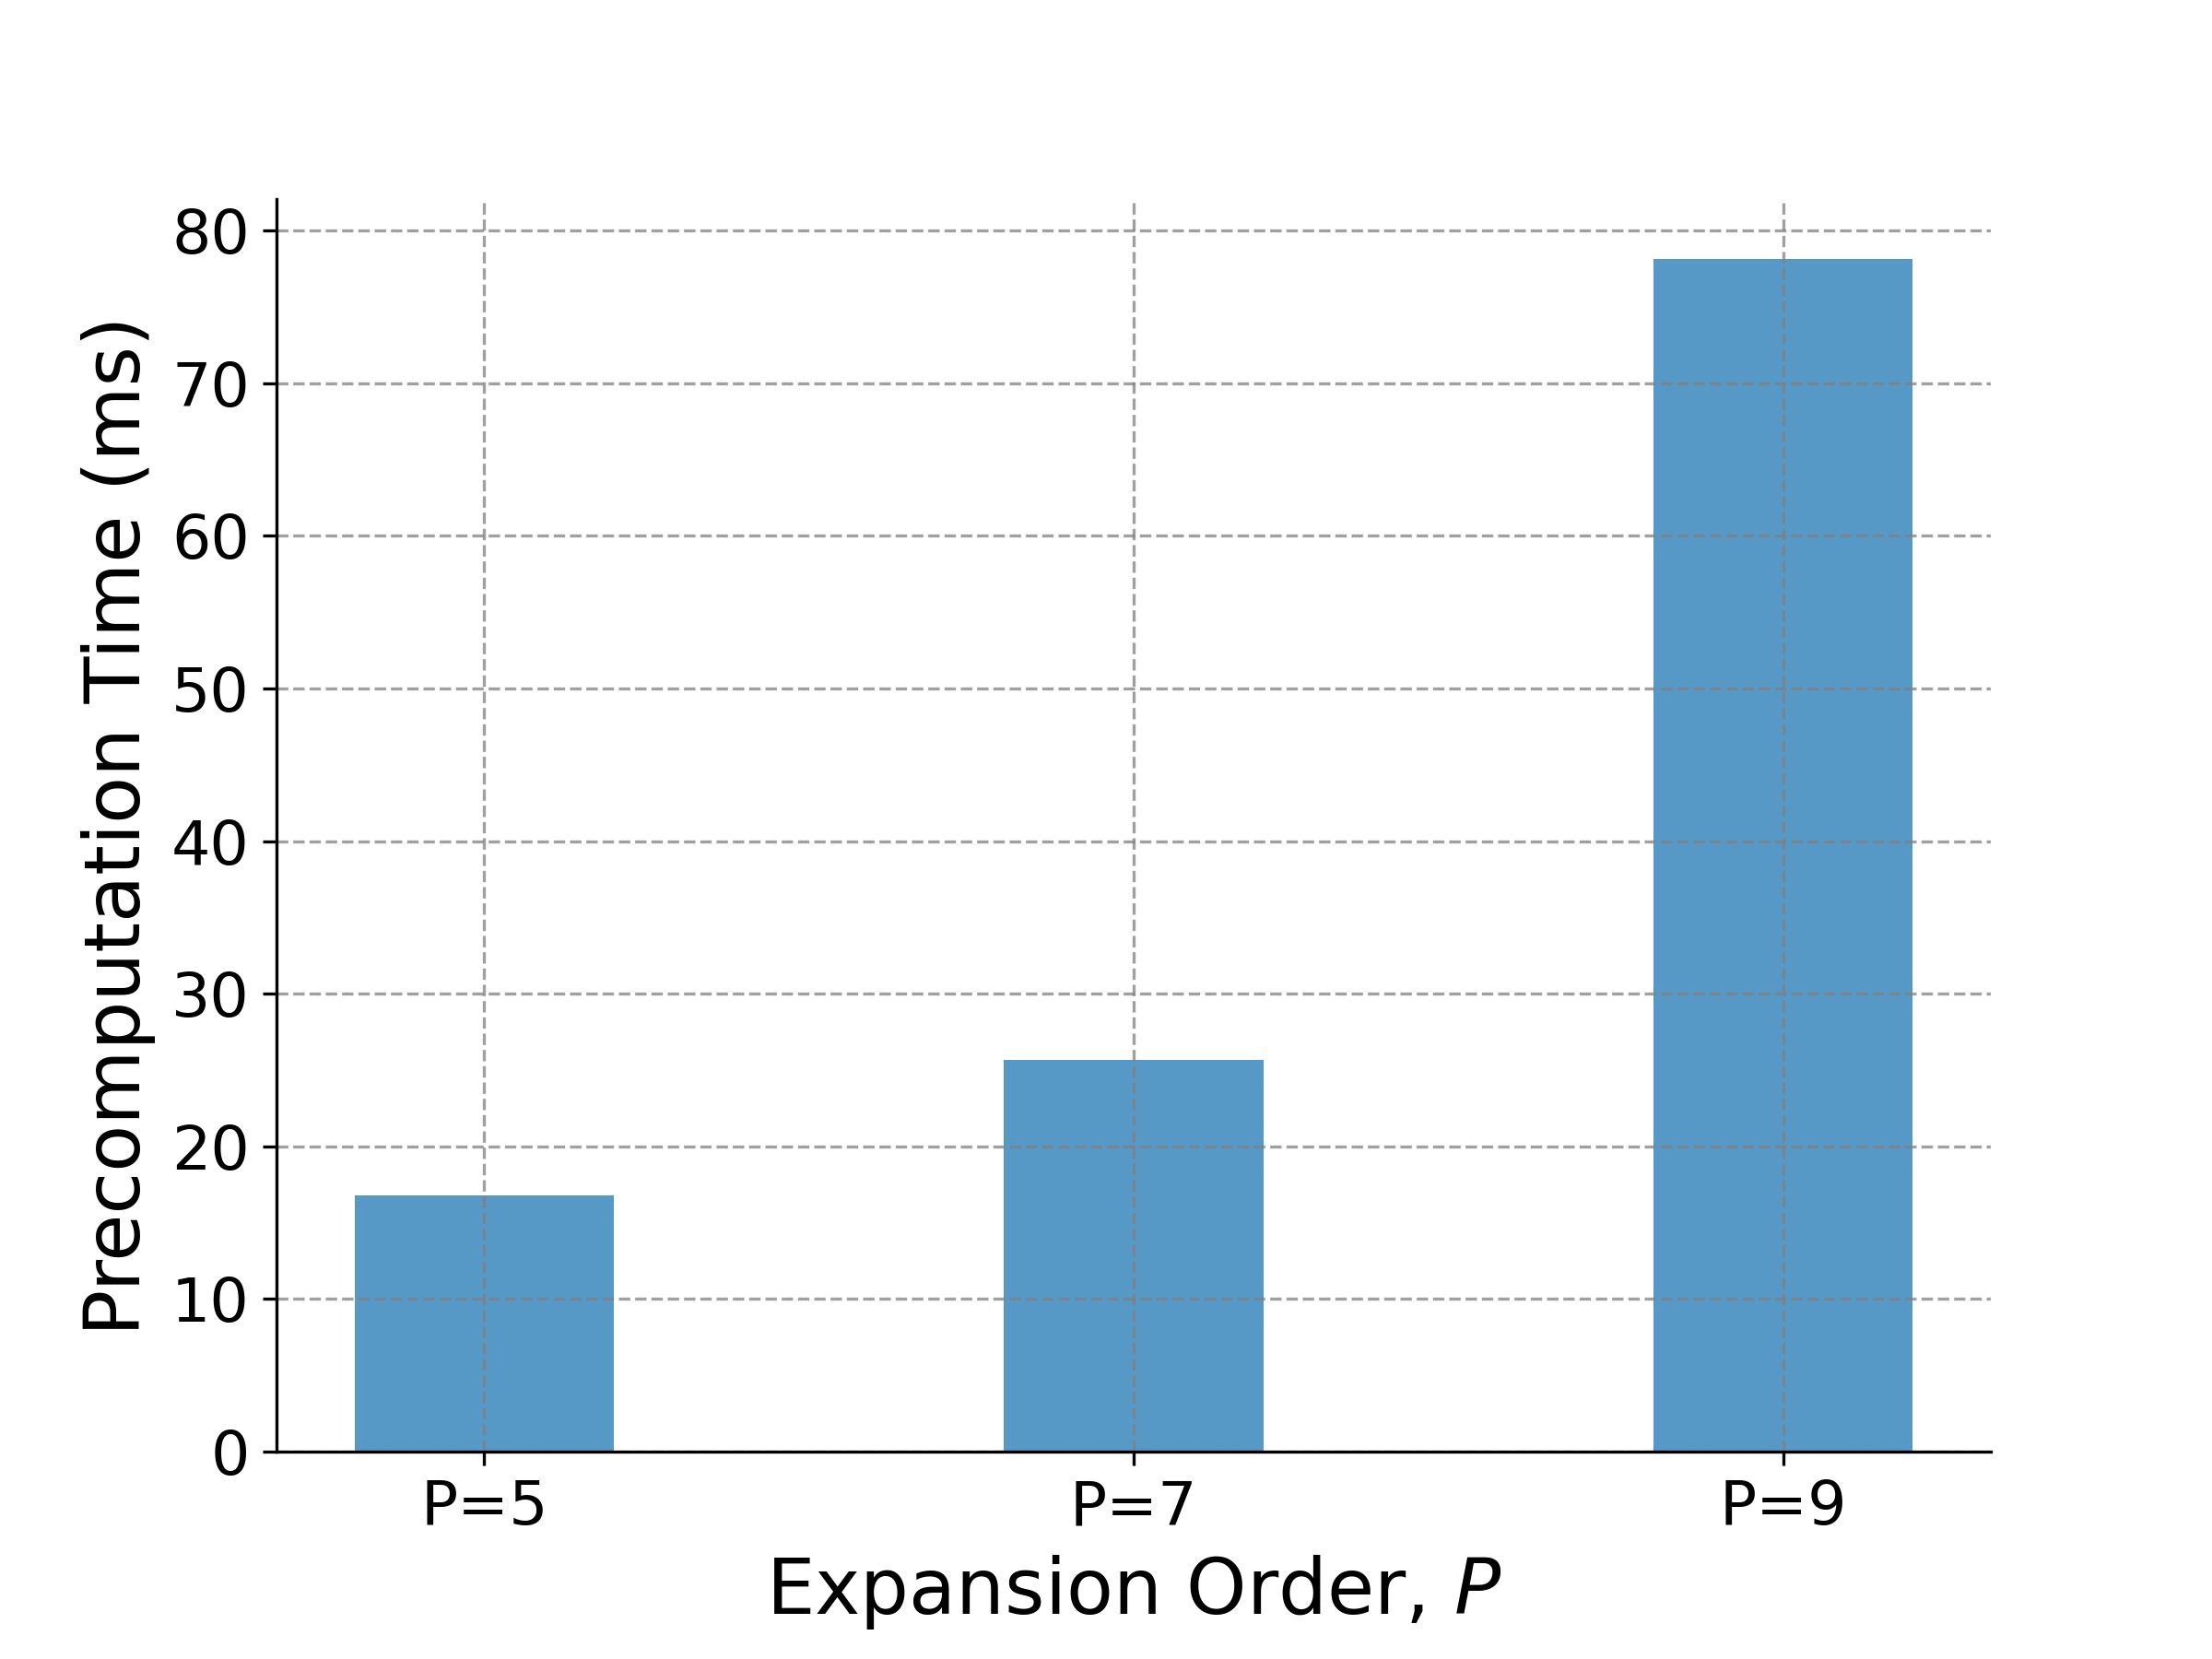
\includegraphics[width=0.6\textwidth]{images/ch_3/fft_m2l_precomputation.png}
    \caption{Here we illustrate the precomputation time to compute the FFTs required of $T^{M2L}$ for a selection of expansion orders for all 316 unique transfer vectors for the Laplace kernel. We highlight the approximately 500x runtime advantage over the precomputations required for the SVD implementation (fig. \ref{fig:chpt:3:sec:1:subsec:1:svd_m2l_precomputation}). Experiments are taken on a 6 core Intel i7-9750 processor using Open BLAS, we report maximum runtimes over 5 runs
    for each set of parameters.}
    \label{fig:chpt:3:sec:1:subsec:2:fft_m2l_precomputation}
\end{figure}\label{chpt:3:sec:1:m2l}

    \chapter{Conclusion}\label{chpt:conclusion}

In this subsidiary thesis we've presented progress on the development of a new software infrastructure for fast algorithms. We've documented recent outputs towards this goal including foundational software as well as a algorithmic techniques. The main outputs being an investigation into programming languages and environments most suitable for scientific computing, a parallel load balanced octree library designed for high-performance,  as well as a proxy-compression based fast direct solver for acoustic Helmholtz scattering problems.

The immediate next steps of this project will be to publish our recent software results on octrees in an appropriate scientific journal. We also intend to continue the developments on fast direct solvers for oscillatory problems, and extend the RS-S framework to electromagnetic scattering problems described by Maxwell's equations. This would constitute a first fast direct solver for electromagnetic scattering problems. In the medium term, we plan to complete the implementation of the parallel FMM software, and the apply this to large scale boundary integral equation problems. This would entail the completion of the majority of our fast solver infrastructure. The final stage of this project will be the extension of our infrastructure to a parallel fast direct solver, and the simulation of large scale electromagnetic scattering problems.
 
    \appendix
    \chapter{Appendix}

\section{Fast Multipole Method Algorithm}\label{app:a_1_fmm_algorithm}

FMM Algorithm logic as pseudocode.


    \printglossary
    \printbibliography[heading=bibintoc]

\end{document}